\documentclass[lettersize,journal]{IEEEtran}
%% ---- Core IEEE / Math ----
\usepackage{amsmath,amsfonts}
\usepackage{mathtools}
\usepackage{mathrsfs}
\usepackage{amsthm}
%% ---- Tables ----
\usepackage{array}
\usepackage{multirow}
\usepackage{booktabs}
\usepackage{makecell}
\usepackage{colortbl}
\usepackage{siunitx}
%% ---- Figures / Subfigures ----
\usepackage{graphicx}
\usepackage[caption=false,font=normalsize,labelfont=sf,textfont=sf]{subfig}
\usepackage{adjustbox}
\usepackage{float}
\usepackage{tikz}
\usetikzlibrary{patterns}
%% ---- Algorithms ----
\usepackage{algorithmic}
\usepackage[linesnumbered,ruled,vlined]{algorithm2e}
%% ---- Code Listings ----
\usepackage{listings}
\usepackage{fancyvrb}
\usepackage{verbatim}
%% ---- Text / Formatting ----
\usepackage[utf8]{inputenc}
\usepackage{textcomp}
\usepackage{xcolor}
\usepackage{pifont}
\usepackage{enumitem}
\usepackage{url}
\usepackage{cite}
\usepackage{balance}
\usepackage{stfloats}
\usepackage{needspace}
\usepackage{microtype}
\usepackage{tcolorbox}
\tcbuselibrary{skins}
\makeatletter
\setlength{\@dblfptop}{0pt}
\makeatother
%% ---- Double-column math adaptation ----
\allowdisplaybreaks
%% ---- Hyphenation hints ----
\hyphenation{op-tical net-works semi-conduc-tor IEEE-Xplore}
%% ---- Custom commands ----
\newcommand{\xmark}{\ding{55}}
\newcommand{\vst}{\textbf{VST User Assertions}}
\newcommand{\acsl}{\textbf{ACSL}}
\newcommand{\defterm}[1]{\textbf{#1}}
\newcommand{\wsl}[1]{{#1}}
\newcommand{\yfp}[1]{{\color{blue} #1}}
\newcommand{\oomit}[1]{}
\newcommand{\statef}{\texttt{StateForm}}
\newcommand{\toolname}{\textsc{SESpec}}
\newcommand{\autospec}{\textsc{AutoSpec}}
\newcommand{\specgen}{\textsc{SpecGen}}
%% ---- Prompt-box style (used by Section IV and Appendix) ----
\lstdefinestyle{PromptBox}{
  basicstyle=\ttfamily\fontsize{6.5}{7.0}\selectfont,
  breaklines=true,
  breakatwhitespace=true,
  breakindent=0pt,
  postbreak=\mbox{\textcolor{gray}{\(\hookrightarrow\)}\space},
  columns=fullflexible,
  keepspaces=true,
  upquote=true,
  literate={`}{{\textasciigrave}}1,
  frame=single,
  framerule=0.4pt,
  framesep=4pt,
  rulecolor=\color{gray!60},
  backgroundcolor=\color{gray!6},
  xleftmargin=1.5mm,
  xrightmargin=1.5mm,
  aboveskip=0.3em,
  belowskip=0.3em,
  escapeinside={(*@}{@*)}
}
% PromptNoBreak: keep the listing as one minipage so it never crosses
% a column/page edge.
\newenvironment{PromptNoBreak}
  {\par\vspace{0.55em}\noindent\begin{minipage}{\linewidth}}
  {\end{minipage}\par\vspace{0.35em}}
% Use \PromptSubsection{...}{label} to emit an appendix subsection that
% reserves enough vertical space so the title and its prompt box stay
% in the same column.
\newcommand{\PromptSubsection}[2]{%
  \Needspace*{12\baselineskip}%
  \subsection{#1}%
  \label{#2}%
}
\newcommand{\PromptSubsubsection}[2]{%
  \Needspace*{12\baselineskip}%
  \subsubsection{#1}%
  \label{#2}%
}
\newcommand{\DiffTag}[2]{\begingroup\setlength{\fboxsep}{1pt}\colorbox{#1!15}{\textcolor{#1!75!black}{\scriptsize\textbf{#2}}}\endgroup}
\newcommand{\circled}[1]{%
  \tikz[baseline=(char.base)]{%
    \node[shape=circle,draw,inner sep=1pt] (char) {#1};%
  }%
}
\newcommand{\fitalign}[1]{%
  \resizebox{\columnwidth}{!}{\parbox{\textwidth}{#1}}%
}
\newcommand{\smallalign}{\small}
\newcommand{\tablefont}{\footnotesize\normalfont}
%% ---- Custom colors ----
\definecolor{myblue}{HTML}{C4DDF5}
\definecolor{myred}{HTML}{F7B6B6}
\definecolor{GPTGreen}{rgb}{0.459,0.675,0.616}
\definecolor{Green}{rgb}{0,0.5,0}
\definecolor{Blue}{rgb}{0.035, 0.682, 0.855}
\definecolor{gray}{rgb}{0.5, 0.5, 0.5}
\definecolor{figgraytext}{HTML}{4D5157}
\definecolor{figgray}{HTML}{7C828A}
\definecolor{figgrayframe}{HTML}{B6BBC1}
\definecolor{figgrayfill}{HTML}{F3F4F6}
\definecolor{figloop}{HTML}{C4DDF5}
\definecolor{figloopstroke}{HTML}{B7D9F4}
\definecolor{figloopfill}{HTML}{F4FAFF}
\definecolor{figcontract}{HTML}{F7B6B6}
\definecolor{figcontractstroke}{HTML}{F4B5B5}
\definecolor{figcontractfill}{HTML}{FFF1F1}
\definecolor{figcall}{HTML}{C7B2DF}
\definecolor{figcallstroke}{HTML}{C4ADDE}
\definecolor{figcallfill}{HTML}{F5EFFA}
\definecolor{overviewgray}{HTML}{F5F5F5}
\definecolor{prompttitlegray}{HTML}{858585}
\definecolor{promptframegray}{HTML}{9A9A9A}
\definecolor{promptbackgray}{HTML}{FBFBFB}
\definecolor{promptblueback}{HTML}{F4FAFF}
\definecolor{promptblueframe}{HTML}{C8DAEE}
\definecolor{promptbluetitle}{HTML}{86A9CE}
\tikzset{
  figaxis/.style={draw=figgrayframe, line width=0.35pt},
  figgrid/.style={draw=figgrayframe!40, line width=0.25pt},
  figbar/.style={rounded corners=1.1pt, draw=none},
  figbarframe/.style={draw=figgrayframe!80, line width=0.28pt, rounded corners=1.1pt}
}
\newcommand{\heat}[1]{%
  \cellcolor{myblue!\numexpr#1\relax!white}{#1\%}%
}
%% ---- Pretty prompt box (tcolorbox + inner listing) ----
\lstdefinestyle{PromptInner}{
  basicstyle=\ttfamily\fontsize{7}{8.4}\selectfont,
  breaklines=true,
  breakatwhitespace=true,
  breakindent=0pt,
  postbreak=\mbox{\textcolor{gray}{$\hookrightarrow$}\space},
  columns=fullflexible,
  keepspaces=true,
  upquote=true,
  literate={`}{{\textasciigrave}}1,
  aboveskip=0pt,
  belowskip=0pt,
  escapeinside={(*@}{@*)}
}
\lstdefinestyle{PromptInnerCompact}{
  style=PromptInner,
  basicstyle=\ttfamily\fontsize{5.8}{6.3}\selectfont
}
%% ---- Case-study code styles (used by the case section and Appendix) ----
\lstdefinestyle{casecodestyle}{
  language=C,
  basicstyle=\ttfamily\fontsize{7pt}{7.4pt}\selectfont,
  keywordstyle=\color{figgraytext}\bfseries,
  keywordstyle=[2]\color{figcontract!80!black}\bfseries,
  keywordstyle=[3]\color{figloop!75!black}\bfseries,
  commentstyle=\color{figcontract!78!black},
  stringstyle=\color{figgraytext},
  identifierstyle=\color{black},
  morekeywords=[2]{requires,ensures,assigns,logic,integer,assert,valid,separated,result,old,at,Pre,true,nothing,decreases},
  morekeywords=[3]{loop,invariant},
  emph={AutoSpec,SESpec,unknown,product,Fib,gcd,gcd_logic,malloc,free},
  emphstyle=\color{figcall!75!black},
  backgroundcolor=\color{overviewgray},
  frame=single,
  frameround=tttt,
  rulecolor=\color{figgrayframe},
  framerule=1pt,
  xleftmargin=1mm,
  xrightmargin=1mm,
  framexleftmargin=1mm,
  framexrightmargin=1mm,
  breaklines=true,
  breakatwhitespace=false,
  columns=fullflexible,
  keepspaces=true,
  showstringspaces=false,
  aboveskip=0pt,
  belowskip=0pt
}
\lstdefinestyle{casecompactstyle}{
  style=casecodestyle,
  basicstyle=\ttfamily\fontsize{5pt}{5.3pt}\selectfont,
  xleftmargin=0.5mm,
  xrightmargin=0.5mm,
  framexleftmargin=0.5mm,
  framexrightmargin=0.5mm
}
\lstdefinestyle{caseinnerstyle}{
  style=casecodestyle,
  frame=none,
  backgroundcolor=\color{overviewgray},
  rulecolor=\color{overviewgray},
  xleftmargin=0pt,
  xrightmargin=0pt,
  framexleftmargin=0pt,
  framexrightmargin=0pt
}
\lstdefinestyle{casecompactinnerstyle}{
  style=casecompactstyle,
  frame=none,
  backgroundcolor=\color{overviewgray},
  rulecolor=\color{overviewgray},
  xleftmargin=0pt,
  xrightmargin=0pt,
  framexleftmargin=0pt,
  framexrightmargin=0pt
}
\tcbset{promptbox/.style={
  enhanced,
  colback=promptblueback,
  colframe=promptblueframe,
  colbacktitle=promptbluetitle,
  coltitle=white,
  boxrule=0.45pt,
  arc=2pt,
  left=5pt, right=5pt, top=4pt, bottom=4pt,
  before skip=8pt plus 2pt minus 2pt,
  after skip=8pt plus 2pt minus 2pt,
  fonttitle=\rmfamily\bfseries\footnotesize,
  titlerule=0pt,
  toptitle=2pt,
  bottomtitle=2pt,
  boxed title style={empty}
}}
\tcbset{promptboxcompact/.style={
  promptbox,
  boxrule=0.4pt,
  left=4pt, right=4pt, top=3pt, bottom=3pt,
  before skip=6pt plus 2pt minus 1pt,
  after skip=6pt plus 2pt minus 1pt,
  fonttitle=\rmfamily\bfseries\scriptsize
}}
\tcbset{casebox/.style={
  promptboxcompact,
  colback=overviewgray,
  colframe=gray!55,
  colbacktitle=gray!75,
  width=\linewidth,
  before skip=5pt plus 1pt minus 1pt,
  after skip=5pt plus 1pt minus 1pt
}}
\newtcolorbox{finding}{enhanced, colback=overviewgray, colframe=gray!55,
  boxrule=0.5pt, arc=2pt, left=6pt, right=6pt, top=3pt, bottom=3pt,
  fontupper=\small, borderline west={2.5pt}{0pt}{gray!80!black}}
%% ---- List / table spacing ----
\AtBeginEnvironment{tabular}{\tablefont}
\AtBeginEnvironment{tabular*}{\tablefont}
\renewcommand{\arraystretch}{1.03}
\setlist[itemize]{noitemsep, topsep=0pt}
%% ---- Float / caption / display spacing (layout only) ----
\setlength{\textfloatsep}{12pt plus 2pt minus 3pt}
\setlength{\dbltextfloatsep}{9pt plus 2pt minus 2pt}
\setlength{\intextsep}{8pt plus 2pt minus 2pt}
\setlength{\floatsep}{8pt plus 2pt minus 2pt}
\setlength{\abovecaptionskip}{5pt}
\setlength{\abovedisplayskip}{1.2ex plus 2pt minus 1pt}
\setlength{\belowdisplayskip}{1.2ex plus 2pt minus 1pt}
\setlength{\abovedisplayshortskip}{0.6ex plus 2pt}
\setlength{\belowdisplayshortskip}{0.6ex plus 2pt}
%% ---- Theorems ----
\newtheorem{definition}{Definition}
\newtheorem{theorem}{Theorem}
\newtheorem{proposition}{Proposition}
%% ---- BibTeX logo ----
\def\BibTeX{{\rm B\kern-.05em{\sc i\kern-.025em b}\kern-.08em
    T\kern-.1667em\lower.7ex\hbox{E}\kern-.125emX}}

%% ---- Hyperlinks and appendix cross-references ----
\usepackage[hidelinks]{hyperref}
\newcommand{\appref}[1]{Appendix~\ref{#1}}
\newcommand{\apptworef}[2]{Appendices~\ref{#1} and~\ref{#2}}
\newcommand{\supref}[1]{\ref{#1}}

% Main-body labels and bibliography numbers are shared with main.pdf.
% Generated cross-document labels pointing to main.pdf.
% Refresh with build_pdfs.sh after structural edits.
\newlabel{sec:intro}{{I}{1}{Introduction}{section.1}{main.pdf}}
\newlabel{sec:motivation}{{II}{2}{A Motivating Example and Our Approach}{section.2}{main.pdf}}
\newlabel{fig:example}{{1}{3}{Motivating Example}{figure.1}{main.pdf}}
\newlabel{fig:overallarchitecture}{{2}{3}{Overview of Our Approach}{figure.2}{main.pdf}}
\newlabel{sec:summarygeneration}{{III}{4}{Pre-/Postcondition Generation}{section.3}{main.pdf}}
\newlabel{sec:default-pre}{{\mbox  {III-B}}{5}{Default Precondition Generation}{subsection.3.2}{main.pdf}}
\newlabel{sec:functionsummary}{{\mbox  {III-C}}{5}{Function Specification Generation Algorithm}{subsection.3.3}{main.pdf}}
\newlabel{alg:funspec-gen}{{1}{5}{Function Specification Generation Algorithm}{algocf.1}{main.pdf}}
\newlabel{sec:llm-fallback}{{\mbox  {III-D}}{6}{LLM Fallback}{subsection.3.4}{main.pdf}}
\newlabel{sec:loopinvariant}{{IV}{6}{Loop Invariant Generation}{section.4}{main.pdf}}
\newlabel{Def:invariant}{{2}{6}{}{definition.2}{main.pdf}}
\newlabel{sec:template}{{\mbox  {IV-B}}{6}{Template Generation}{subsection.4.2}{main.pdf}}
\newlabel{sec:refinement}{{\mbox  {IV-C}}{7}{Verifier-Guided Specification Refinement}{subsection.4.3}{main.pdf}}
\newlabel{sec:experiments}{{V}{7}{Experiments}{section.5}{main.pdf}}
\newlabel{tab:dataset_overview}{{I}{8}{Dataset overview by program type}{table.1}{main.pdf}}
\newlabel{tab:performance_rates_model}{{II}{8}{Specification generation performance under Pass@1 and Pass@5. The complete Pass@1/3/5 table is given in Table~\supref {tab:performance_rates_model_full} (\appref {app:rq2-full})}{table.2}{main.pdf}}
\newlabel{tab:ablation}{{III}{9}{Ablation study}{table.3}{main.pdf}}
\newlabel{sec:inv_experiments}{{\mbox  {V-E}}{9}{RQ4: Does \toolname \ outperform LLM- and SMT-based baselines?}{subsection.5.5}{main.pdf}}
\newlabel{sec:large-scale-experiment}{{VI}{9}{Goal-Independent Evaluation}{section.6}{main.pdf}}
\newlabel{subsec:rq5-valid}{{\mbox  {VI-B}}{9}{RQ5: How often does \toolname \ produce a \emph {Valid} specification?}{subsection.6.2}{main.pdf}}
\newlabel{tab:comparison}{{IV}{10}{Accuracy comparison across benchmarks and baselines. \toolname \ reports Pass@5 (cf.\ Table~\ref {tab:performance_rates_model}); baselines use their best reported configuration}{table.4}{main.pdf}}
\newlabel{tab:large_experiment_summary}{{V}{10}{Native-verifier validity on \toolname -400}{table.5}{main.pdf}}
\newlabel{subsec:rq6-strength}{{\mbox  {VI-C}}{10}{RQ6: How strong are \toolname 's specifications versus the baselines?}{subsection.6.3}{main.pdf}}
\newlabel{fig:fc_vs_judge_strength}{{3}{11}{Dimension-wise relations for \autospec \ versus \toolname \ over identical data sets. A directional segment means a more permissive accepted domain for preconditions and a logically stronger predicate for postconditions or invariants. ``Judge + expert'' is the corrected judge result; WP checks the same implications. Right-hand counts follow the legend order}{figure.3}{main.pdf}}
\newlabel{subsec:rq7-cost}{{\mbox  {VI-D}}{11}{RQ7: What does \toolname \ cost in time, tokens, API calls, and memory?}{subsection.6.4}{main.pdf}}
\newlabel{subsec:rq8-failure}{{\mbox  {VI-E}}{11}{RQ8: What are \toolname 's dominant failure modes?}{subsection.6.5}{main.pdf}}
\newlabel{sec:relatedwork}{{VII}{11}{Related Work}{section.7}{main.pdf}}
\newlabel{fig:rq7-cost}{{4}{12}{Mean cost per attempted program on all 400 \texttt {gpt-5.4-mini} cases. Each bar stacks valid-run (solid) and failed-run (hatched) contributions, each divided by 400}{figure.4}{main.pdf}}
\newlabel{fig:failure_root_causes}{{5}{12}{Failure outcome and root-cause summary for the \texttt {gpt-5.4-mini} \toolname -400 rerun}{figure.5}{main.pdf}}
\newlabel{sec:conclusion}{{VIII}{12}{Conclusion}{section.8}{main.pdf}}
\newlabel{tab:positioning}{{VI}{13}{Positioning of \toolname \ against representative specification and invariant generation tools}{table.6}{main.pdf}}

% Citation numbers shared with main.pdf; links open its bibliography.
\makeatletter
\expandafter\gdef\csname b@DBLP:conf/cav/ColonSS03\endcsname{%
  \hyper@@link[cite]{main.pdf}{cite.DBLP:conf/cav/ColonSS03}{1}}
\expandafter\gdef\csname b@DBLP:journals/pacmpl/LiuFYSL22\endcsname{%
  \hyper@@link[cite]{main.pdf}{cite.DBLP:journals/pacmpl/LiuFYSL22}{2}}
\expandafter\gdef\csname b@FiB_Squeezing_loop\endcsname{%
  \hyper@@link[cite]{main.pdf}{cite.FiB_Squeezing_loop}{3}}
\expandafter\gdef\csname b@DBLP:conf/cade/GanDXZKC16\endcsname{%
  \hyper@@link[cite]{main.pdf}{cite.DBLP:conf/cade/GanDXZKC16}{4}}
\expandafter\gdef\csname b@Nonlinear_Craig_Interpolant_Generation\endcsname{%
  \hyper@@link[cite]{main.pdf}{cite.Nonlinear_Craig_Interpolant_Generation}{5}}
\expandafter\gdef\csname b@beyer2024decomposing\endcsname{%
  \hyper@@link[cite]{main.pdf}{cite.beyer2024decomposing}{6}}
\expandafter\gdef\csname b@wonisch2012predicate\endcsname{%
  \hyper@@link[cite]{main.pdf}{cite.wonisch2012predicate}{7}}
\expandafter\gdef\csname b@calcagno2009compositional\endcsname{%
  \hyper@@link[cite]{main.pdf}{cite.calcagno2009compositional}{8}}
\expandafter\gdef\csname b@Daikon\endcsname{%
  \hyper@@link[cite]{main.pdf}{cite.Daikon}{9}}
\expandafter\gdef\csname b@Code2Inv_a_Deep_Learning_Framework_for_Program_Verification\endcsname{%
  \hyper@@link[cite]{main.pdf}{cite.Code2Inv_a_Deep_Learning_Framework_for_Program_Verification}{10}}
\expandafter\gdef\csname b@Loop_Invariant_Inference_through_SMT_Solving_Enhanced_Reinforcement_Learning\endcsname{%
  \hyper@@link[cite]{main.pdf}{cite.Loop_Invariant_Inference_through_SMT_Solving_Enhanced_Reinforcement_Learning}{11}}
\expandafter\gdef\csname b@DBLP:journals/pacmse/CaoWXYWCM25\endcsname{%
  \hyper@@link[cite]{main.pdf}{cite.DBLP:journals/pacmse/CaoWXYWCM25}{12}}
\expandafter\gdef\csname b@autospec\endcsname{%
  \hyper@@link[cite]{main.pdf}{cite.autospec}{13}}
\expandafter\gdef\csname b@Enhancing_Automated_Loop_Invariant_Generation_for_Complex_Programs_with_Large_Language_Models\endcsname{%
  \hyper@@link[cite]{main.pdf}{cite.Enhancing_Automated_Loop_Invariant_Generation_for_Complex_Programs_with_Large_Language_Models}{14}}
\expandafter\gdef\csname b@SpecGen\endcsname{%
  \hyper@@link[cite]{main.pdf}{cite.SpecGen}{15}}
\expandafter\gdef\csname b@Wang2025ATO\endcsname{%
  \hyper@@link[cite]{main.pdf}{cite.Wang2025ATO}{16}}
\expandafter\gdef\csname b@vst-a\endcsname{%
  \hyper@@link[cite]{main.pdf}{cite.vst-a}{17}}
\expandafter\gdef\csname b@wu2025qcppracticalseparationlogicbased\endcsname{%
  \hyper@@link[cite]{main.pdf}{cite.wu2025qcppracticalseparationlogicbased}{18}}
\expandafter\gdef\csname b@cuoq2012frama\endcsname{%
  \hyper@@link[cite]{main.pdf}{cite.cuoq2012frama}{19}}
\expandafter\gdef\csname b@alur2019sygus\endcsname{%
  \hyper@@link[cite]{main.pdf}{cite.alur2019sygus}{20}}
\expandafter\gdef\csname b@Inductive_Invariant_Generation_via_Abductive_Inference\endcsname{%
  \hyper@@link[cite]{main.pdf}{cite.Inductive_Invariant_Generation_via_Abductive_Inference}{21}}
\expandafter\gdef\csname b@LIG-MM\endcsname{%
  \hyper@@link[cite]{main.pdf}{cite.LIG-MM}{22}}
\expandafter\gdef\csname b@le2025can\endcsname{%
  \hyper@@link[cite]{main.pdf}{cite.le2025can}{23}}
\expandafter\gdef\csname b@A_Data_Driven_Approach_for_Algebraic_Loop\endcsname{%
  \hyper@@link[cite]{main.pdf}{cite.A_Data_Driven_Approach_for_Algebraic_Loop}{24}}
\expandafter\gdef\csname b@dig\endcsname{%
  \hyper@@link[cite]{main.pdf}{cite.dig}{25}}
\expandafter\gdef\csname b@Abstract_Interpretation_A_Unified_Lattice_Model_for_Static_Analysis_of_Programs_by_Construction_or_Approximation_of_Fixpoints\endcsname{%
  \hyper@@link[cite]{main.pdf}{cite.Abstract_Interpretation_A_Unified_Lattice_Model_for_Static_Analysis_of_Programs_by_Construction_or_Approximation_of_Fixpoints}{26}}
\expandafter\gdef\csname b@Automatic_Discovery_of_Linear_Restraints_among_Variables_of_a_Program\endcsname{%
  \hyper@@link[cite]{main.pdf}{cite.Automatic_Discovery_of_Linear_Restraints_among_Variables_of_a_Program}{27}}
\expandafter\gdef\csname b@ISSACDeepakKapur\endcsname{%
  \hyper@@link[cite]{main.pdf}{cite.ISSACDeepakKapur}{28}}
\expandafter\gdef\csname b@DBLP:journals/jsc/Rodriguez-CarbonellK07\endcsname{%
  \hyper@@link[cite]{main.pdf}{cite.DBLP:journals/jsc/Rodriguez-CarbonellK07}{29}}
\expandafter\gdef\csname b@DBLP:journals/pacmpl/CyphertK24\endcsname{%
  \hyper@@link[cite]{main.pdf}{cite.DBLP:journals/pacmpl/CyphertK24}{30}}
\expandafter\gdef\csname b@Backward_Symbolic_Execution_with_Loop_Folding\endcsname{%
  \hyper@@link[cite]{main.pdf}{cite.Backward_Symbolic_Execution_with_Loop_Folding}{31}}
\expandafter\gdef\csname b@SymInfer_Inferring_Numerical_Invariants_using_Symbolic_States\endcsname{%
  \hyper@@link[cite]{main.pdf}{cite.SymInfer_Inferring_Numerical_Invariants_using_Symbolic_States}{32}}
\expandafter\gdef\csname b@Synthesizing_Invariants_for_Polynomial_Programs_by_Semidefinite_Programming\endcsname{%
  \hyper@@link[cite]{main.pdf}{cite.Synthesizing_Invariants_for_Polynomial_Programs_by_Semidefinite_Programming}{33}}
\expandafter\gdef\csname b@Counterexample_Guided_Inductive_Synthesis_Modulo_Theories\endcsname{%
  \hyper@@link[cite]{main.pdf}{cite.Counterexample_Guided_Inductive_Synthesis_Modulo_Theories}{34}}
\expandafter\gdef\csname b@Ryan2020CLN2INV\endcsname{%
  \hyper@@link[cite]{main.pdf}{cite.Ryan2020CLN2INV}{35}}
\expandafter\gdef\csname b@iRank\endcsname{%
  \hyper@@link[cite]{main.pdf}{cite.iRank}{36}}
\expandafter\gdef\csname b@Lemur\endcsname{%
  \hyper@@link[cite]{main.pdf}{cite.Lemur}{37}}
\expandafter\gdef\csname b@LLM_Generated_Invariants_for_Bounded_Model_Checking_Without_Loop_Unrolling\endcsname{%
  \hyper@@link[cite]{main.pdf}{cite.LLM_Generated_Invariants_for_Bounded_Model_Checking_Without_Loop_Unrolling}{38}}
\expandafter\gdef\csname b@kamath2023findinginductiveloopinvariants\endcsname{%
  \hyper@@link[cite]{main.pdf}{cite.kamath2023findinginductiveloopinvariants}{39}}
\expandafter\gdef\csname b@Can_Large_Language_Models_Reason_About_Program_Invariants\endcsname{%
  \hyper@@link[cite]{main.pdf}{cite.Can_Large_Language_Models_Reason_About_Program_Invariants}{40}}
\expandafter\gdef\csname b@thakur2025clever\endcsname{%
  \hyper@@link[cite]{main.pdf}{cite.thakur2025clever}{41}}
\expandafter\gdef\csname b@ye2026verina\endcsname{%
  \hyper@@link[cite]{main.pdf}{cite.ye2026verina}{42}}
\expandafter\gdef\csname b@DBLP:conf/osdi/CadarDE08\endcsname{%
  \hyper@@link[cite]{main.pdf}{cite.DBLP:conf/osdi/CadarDE08}{43}}
\expandafter\gdef\csname b@kuznetsov2012merging\endcsname{%
  \hyper@@link[cite]{main.pdf}{cite.kuznetsov2012merging}{44}}
\expandafter\gdef\csname b@avgerinos2014veritesting\endcsname{%
  \hyper@@link[cite]{main.pdf}{cite.avgerinos2014veritesting}{45}}
\expandafter\gdef\csname b@yang2026how\endcsname{%
  \hyper@@link[cite]{main.pdf}{cite.yang2026how}{46}}
\expandafter\gdef\csname b@li2026goedelcodeproverhierarchicalproofsearch\endcsname{%
  \hyper@@link[cite]{main.pdf}{cite.li2026goedelcodeproverhierarchicalproofsearch}{47}}
\makeatother



\newcommand{\wslcomment}[1]{{\color{blue} wsl:#1}}

\begin{document}
% Resume the numbering used by the complete whole.tex document.
\setcounter{figure}{5}
\setcounter{table}{6}
\setcounter{algocf}{1}
\setcounter{equation}{0}
\setcounter{definition}{2}
\setcounter{theorem}{0}
\setcounter{proposition}{0}

\appendices
\raggedbottom
\section{Proof of the Strongest-Postcondition Guarantee}
\label{app:sp-proof}

{We first restate the proposition from Section~\ref{sec:summarygeneration} and then give its proof.}

\begin{proposition}
\label{thm:sp-sound-complete}
 $\textit{SP}(\mathcal{F},P,p_{\textit{start}},p_{\textit{end}})$ is the \emph{strongest postcondition} of $\mathcal{F}$ with respect to $P$, if the following conditions hold:
 \begin{itemize}
     \item[(A1)] Scope conditions: $\mathcal{F}$ contains no external calls (i.e., every called function has a definition), no loops, and every memory access is representable in the flattened model. {For every input satisfying $P$, execution of the interval is well-defined under the modeled C semantics: memory accesses, aliasing, and arithmetic operations are represented exactly and no undefined behavior occurs.}
     \item[(A2)] Symbolic execution conditions: The symbolic execution procedure is path-complete, it enumerates all feasible paths from $p_{\textit{start}}$ to $p_{\textit{end}}$ {under $P$}. Furthermore, for each enumerated path $\pi$, the path condition $PC_\pi$ exactly characterizes the inputs that cause the concrete execution to follow $\pi$, and the symbolic store $\sigma_{p_{\textit{end}},\pi}$ exactly expresses the resulting concrete state at $p_{\textit{end}}$ in
     terms of the function-entry symbolic values, according to the flattened memory semantics. {These statements concern the common endpoint locations; other endpoint locations are not characterized by the formula.}

     
 \end{itemize}
\end{proposition}

\begin{proof}
    Denote $\textit{SP}(\mathcal{F},P,p_{\textit{start}},p_{\textit{end}})$ by $\Phi$. {We show that its satisfying state pairs are exactly the reachable pairs projected to the common endpoint locations; this establishes both soundness and maximality over those variables.}

    (Soundness): Take any initial state $s_0$ satisfying $P$. Since $\mathcal{F}$ is loop-free and contains no external calls, {and (A1) excludes undefined behavior on this input,} its concrete execution follows a feasible path $\pi$ and reaches $p_{\textit{end}}$ in state $s$. By (A2) path-completeness, symbolic execution enumerates $\pi$. By (A1) and (A2), its flattened-memory transfers agree with the concrete execution on every tracked cell. {Consequently, $PC_\pi$ holds and $\ell^{p_{\textit{end}}}=\sigma_{p_{\textit{end}},\pi}(\ell)$ for every $\ell\in\mathcal L_{p_{\textit{end}}}$ under the pair $(s_0,s)$. Hence this pair satisfies $PC_\pi\land\rho(\sigma_{p_{\textit{end}},\pi}|_{\mathcal L_{p_{\textit{end}}}})$ and therefore $\Phi$. This proves that every reachable pair satisfies $\Phi$.}

    (Completeness): {Let $(s_0,s)$ satisfy $\Phi$. Some feasible path $\pi$ then satisfies $PC_\pi$ and $\rho(\sigma_{p_{\textit{end}},\pi}|_{\mathcal L_{p_{\textit{end}}}})$ under this pair. Since $PC_\pi$ includes $P$, the initial state satisfies $P$. Exact path conditions and transfers in (A2), together with (A1), give a defined concrete execution along $\pi$ whose final state agrees with $s$ on the common endpoint locations. Thus the projected pair is reachable. If $\{P\}\,\mathcal{F}\,\{\Psi\}$ holds for any formula $\Psi$ over the same projected state variables, every reachable projected pair satisfies $\Psi$, so $\Phi\Rightarrow\Psi$. This proves the strongest-postcondition claim.}
\end{proof}

\section{LLM Fallback Details}
\label{app:fallback}

In the fallback, the LLM acts as a semantic summarization component for the missing symbolic‑execution step. It receives the current code fragment, available symbolic states and path conditions, previously generated callee specifications or loop summaries, and an ACSL skeleton. The LLM is tasked with following the relevant paths, tracking changes to variables and memory locations, and proposing ACSL clauses that summarize the observed behavior. The resulting candidates must still be proved by Frama‑C/WP. 

%The fallback uses the LLM as a semantic summarization component for the missing symbolic-execution step, proposing ACSL candidates that must still be proved by Frama-C/WP. It receives the current code fragment, available symbolic states and path conditions, previously generated callee specifications or loop summaries, and an ACSL skeleton, and is instructed to follow the relevant paths, to track changes to variables and memory locations, and to propose ACSL clauses that summarize the observed behavior.

We use this fallback for four function-level tasks. \emph{Precondition generation} asks the LLM to infer candidate \texttt{requires} clauses describing the validity, separation and bound constraints. \emph{Assigns-clause generation} asks the LLM to infer the function's footprint, i.e., \texttt{assigns} clauses describing which visible memory locations may be modified. \emph{Postcondition generation} asks the LLM to summarize the relation between the pre-state and the post-state, filling candidate \texttt{ensures} clauses. \emph{Inductive-predicate generation} asks the LLM to decide whether the program requires an inductive predicate and, when needed, to propose one for capturing inductive relations in recursive data structures or recursive functions.


\section{Loop Analysis Procedure}
\label{app:loop-analysis}

\begin{algorithm}[htbp]
\caption{Loop Analysis $\mathrm{LoopAnalysis}$}
\label{alg:loop-analysis}
\small
\KwIn{loop body $\mathcal{F}_{\textit{loop}}$, precondition $\textit{Pre}$, loop stack $\textit{lS}$, call stack $\textit{cS}$, annotated functions $\textit{aF}$, LLM}
\KwOut{annotated $\mathcal{F}_{\textit{loop}}$, sets of unchanged variables $\textit{uV}$ and non-inductive variables $\textit{nV}$}

$\mathcal{F}_{\textit{unfolded}} \gets \mathrm{UnfoldLoop}(\mathcal{F}_{\textit{loop}})$\;
$P \gets \textit{Pre}$\;
$p_{\textit{start}} \gets p_{\textit{unfolded}\_0}$\;
$p \gets \mathrm{SEStart}(\mathcal{F}_{\textit{unfolded}},P, p_{\textit{start}})$\;

\While{$p \neq p_{\textit{unfolded}\_{-1}}$}{
    $P \gets \textit{SP}(\mathcal{F}_{\textit{unfolded}},P,p_{\textit{start}},p)$\tcp*{\small Same as $\mathrm{FuncSpec}$}
    $p_{\textit{start}} \gets p$\;
    \If{$p = p_{\textit{nestedLoopEntry}}$}{
        $\textit{lS}.\mathrm{push}(\mathcal{F}_{\textit{nested}})$\;
    }
    \If{$p = p_{\textit{nestedLoopExit}}$}{
        $\mathcal{F}_{\textit{nested}} \gets \textit{lS}.\mathrm{pop}()$\;
        $\mathcal{F}_{\textit{loop}} \gets \mathrm{NestedLoopLLMCall}(\mathcal{F}_{\textit{loop}},\mathcal{F}_{\textit{nested}},\textit{LLM})$\;
    }
    \If{$p = p_{\textit{callee}}$}{
        $\mathcal{F}_{\textit{callee}} \gets \mathrm{FuncSpec}(\mathcal{F}_{\textit{callee}},\textit{cS},\textit{aF})$\;
    }
    $p \gets \mathrm{SEStart}(\mathcal{F}_{\textit{unfolded}},P, p_{\textit{start}})$\;
}

$\ldots$\tcp*{\small Same as $\mathrm{FuncSpec}$, construct the final postcondition $\mathcal{S}$}

$\textit{uV} \gets \mathrm{FetchUnchangedVars}(\mathcal{S})$\;
$\textit{nV} \gets \mathrm{FetchNonInductiveVars}(\mathcal{S})$\;

\Return $\mathcal{F}_{\textit{loop}},\textit{uV},\textit{nV}$\;
\end{algorithm}

$\mathrm{LoopAnalysis}$ (Algorithm~\ref{alg:loop-analysis}) symbolically executes a single-iteration unfolding $\mathcal{F}_{\textit{unfolded}}$ of the loop body (Lines~1--4) and then advances through it one program point at a time (Lines~5--15), exposing the update and frame facts of one iteration. The key difference from $\mathrm{FuncSpec}$ lies in the handling of nested loops: whereas the outer loop uses symbolic-execution-derived preconditions and templates to guide LLM synthesis ($\mathrm{OuterLoopLLMCall}$), an inner loop is processed purely through $\mathrm{NestedLoopLLMCall}$ (Lines~10--12), which infers its invariant directly from the code context without preconditions or templates, because a well-defined precondition is not available at the enclosing loop boundary. Nested loops are thus discharged bottom-up using the loop stack $\textit{lS}$, while function calls are handled consistently with $\mathrm{FuncSpec}$ through the call stack $\textit{cS}$ (Lines~13--14): the callee is summarized before symbolic execution of the unfolded body resumes. Once the unfolded body has been fully executed, its final postcondition is constructed and all nested loops are annotated with the invariants generated for them; this postcondition is then used to classify the unchanged variables $\textit{uV}$ and non-inductive variables $\textit{nV}$ of the outer loop (Lines~16--18).

The driving $\mathrm{LoopInvGen}$ procedure (Algorithm~\ref{alg:loopinv-gen}) wraps $\mathrm{LoopAnalysis}$ with template generation ($\mathrm{LoopInvTemGen}$), a single $\mathrm{OuterLoopLLMCall}$, and a verification-and-refine pass.

\begin{algorithm}[htbp]
\caption{Loop Invariant Generation $\mathrm{LoopInvGen}$}
\label{alg:loopinv-gen}
\small
\KwIn{function $\mathcal{F}$, loop entry $p_{\textit{loop}}$, loop stack $\textit{lS}$, call stack $\textit{cS}$, annotated functions $\textit{aF}$, loop precondition $P$, LLM}
\KwOut{function $\mathcal{F}$ annotated with loop invariant $\mathcal{I}$ for the loop $\mathcal{F}_{\textit{loop}}$ at $p_{\textit{loop}}$}

\tcp{\small \textit{$\mathcal{F}_{\textit{loop}}$ is the loop body at $p_{\textit{loop}}$ in $\mathcal{F}$}}
$\mathrm{ThinkInNaturalLanguage}(\mathcal{F}_{\textit{loop}},\textit{LLM})$\;
$\textit{lS}.\mathrm{push}(\mathcal{F}_{\textit{loop}})$\;
$\mathcal{F}_{\textit{loop}}, \textit{uV}, \textit{nV} \gets \mathrm{LoopAnalysis}(\mathcal{F}_{\textit{loop}},P,\textit{lS},\textit{cS},\textit{aF},\textit{LLM})$\;
$\textit{lS}.\mathrm{pop}()$\tcp*{\small \textit{$\textit{lS}$ depth is unchanged across this call}}
$\mathcal{T} \gets \mathrm{LoopInvTemGen}(\mathcal{F}_{\textit{loop}},P,\textit{uV},\textit{nV})$\;
$\mathcal{I} \gets \mathrm{OuterLoopLLMCall}(\mathcal{F},\mathcal{F}_{\textit{loop}},P,\mathcal{T},\textit{LLM})$\;
$\mathcal{F} \gets (\mathcal{F},\mathcal{I})$\;

\If{$\neg \mathrm{Verify}(\mathcal{F})$}{
    $\mathcal{F} \gets \mathrm{Refine}(\mathcal{F},\mathcal{I},P,\textit{loop},\textit{LLM})$\;
}

\Return $\mathcal{F}$\;
\end{algorithm}

\section{System Design and Prompt Construction}
\label{sec:impl}

\subsection{Execution and Verification Backbone}

The implementation combines three off-the-shelf components: the QCP symbolic execution engine~\cite{wu2025qcppracticalseparationlogicbased,vst-a}, an LLM, and the Frama-C/WP automated verifier~\cite{cuoq2012frama}, and orchestrates them through a thin translation layer. Symbolic execution drives the pipeline and pauses at each loop and function call, where the LLM proposes the missing annotations from the exposed symbolic state and Frama-C/WP discharges the resulting proof obligations.


The choice of QCP and Frama-C is motivated by their complementary strengths. QCP is used as the symbolic execution engine because it produces Coq-verified postconditions and, more importantly, exposes its symbolic state (path conditions plus symbolic stores) at arbitrary program points in a logical form that is directly reusable for specification synthesis. Crucially, QCP satisfies the symbolic-execution conditions of Proposition~\ref{thm:sp-sound-complete}, thereby providing the foundation for the strongest-postcondition guarantee on loop-free segments. Other widely used alternatives such as Klee~\cite{DBLP:conf/osdi/CadarDE08} are not built on Hoare logic and accordingly neither expose intermediate states at arbitrary locations nor present them in a logic-oriented form suitable for specification synthesis. QCP also has strong support for programs that manipulate complex data structures and ships with a library of verified inductive predicates and lemmas, which matches our goal of producing formally precise specifications. The gap QCP leaves --- it requires user-supplied loop invariants and callee pre-/postconditions, and it may emit lemmas that need additional Coq interactive proofs --- is exactly the gap filled by the other two components. The LLM proposes the missing invariants and specifications from the symbolic state QCP exposes; Frama-C/WP then discharges the resulting proof obligations automatically through SMT under the LLM-friendly ACSL surface syntax. The three components therefore split the work cleanly: QCP supplies the symbolic semantics, the LLM supplies the specification candidates, and Frama-C/WP closes the verification loop.

%Stitching these three components together cleanly requires a translation layer, because each of them speaks a different annotation language: QCP consumes and emits QCPL (its native annotation language), the LLM is prompted in ACSL plus natural language, and Frama-C/WP verifies ACSL. The translator maintains a bidirectional bridge between ACSL and QCPL --- forward-translating ACSL clauses into QCPL during the $\mathrm{LoopInvGen}$ phase so that QCP can use them consistently across loop and function boundaries, and back-translating QCP's symbolic-state output into ACSL skeletons (for the LLM, paired with natural-language guidance) and into ACSL clauses (for Frama-C/WP verification). A deliberate design choice is that QCPL is never shown to the LLM: the model only ever sees ACSL plus natural-language guidance derived from the symbolic state. This avoids the well-documented failure mode of an LLM confusing two formally similar but semantically distinct annotation languages, and the skeleton-plus-prose discipline doubles as a pre-structured frame so that structural well-formedness is the translator's responsibility and the model is left to fill in the logical content of each placeholder. When verification fails, error information is translated into natural language together with its original context and routed back into the next LLM call, closing the loop without ever exposing the LLM to the verifier's internal representation either.

Stitching these three components together requires a translation layer, because QCP, the LLM, and Frama‑C/WP each speak a different annotation language: QCPL (native to QCP), ACSL (native to Frama‑C/WP), and natural-language prompts (for the LLM). The translator maintains a bidirectional bridge between ACSL and QCPL: it translates ACSL clauses into QCPL so that QCP can use them across loop and function boundaries, and it converts QCP’s symbolic‑state output into ACSL skeletons (paired with natural‑language guidance for the LLM) and ACSL clauses (for Frama‑C/WP verification). A deliberate design choice is that the LLM never sees QCPL; it only operates on ACSL plus natural‑language guidance derived from the symbolic state. This avoids the common failure mode of confusing two formally similar but semantically distinct languages, and the skeleton‑plus‑prose discipline ensures structural well‑formedness before the LLM fills in the logical content. When verification fails, error information is translated back into natural language, together with its context, and routed into the next LLM call—closing the loop without exposing the verifier’s internal representation to the model either.

\subsection{Prompt Construction}
\label{sec:prompt}

\noindent
Every LLM call in \toolname\ follows a fixed template, but the concrete prompt is specialized to the input program. A lightweight static classifier inspects the source code and assigns each program to one of five routes: recursive data structure, recursive program, array, numeric, and plain, where plain is the default route for programs that do not need helper definitions. The selected route determines which worked examples, category-specific ACSL guidance, and route-specific rule fragments are inserted on top of the universal ACSL pitfalls block. Thus, the same template yields substantively different prompts for, say, a numeric recurrence and a linked-list cursor.

This routing drives the five LLM call sites in the pipeline: loop invariant generation, precondition generation, postcondition/assigns generation, syntax repair, and verifier-guided semantic refinement. In addition, the symbolic executor supplies the state-dependent content of each prompt --- the variable state and the path constraints --- together with an annotation skeleton to be completed by the LLM. At refinement time, the verifier's typed error categories are additionally folded into the prompt. All prompt templates are listed in {Section~\ref{app:prompts}}.

\subsection{Full Prompt Templates}
\label{app:prompts}

This section lists the templates used by the main LLM call sites referenced in Section~\ref{sec:prompt}, abridged to their static skeleton and runtime slots (the verbose in-prompt admonitions are elided). Each template's static body is shown in black; runtime-injected slots appear in gray with colored tags from the shared figure palette: \DiffTag{figloop}{LOOP/SYMBOLIC} for loop-aware symbolic context, \DiffTag{figcall}{ROUTE/CALL} for route and call-site context, and \DiffTag{figcontract}{VERIFIER/SPECIFICATION} for verifier errors and specification edits.


\PromptSubsubsection{Loop-invariant generation}{app:prompt-loop}

The example below is a filled loop-invariant prompt for a small branch-then-loop program, with the long example and guidance blocks elided.

\begin{tcolorbox}[promptboxcompact, title={Loop-invariant generation prompt}]
\begin{lstlisting}[style=PromptInnerCompact]
### Role / Task ###
Given a C program with a loop, generate ACSL loop invariants
that let Frama-C verify it.

(*@\DiffTag{figcall}{ROUTE}\quad{\normalfont\itshape\color{gray!60!black}examples + ACSL helper policy for the matched route, omitted}@*)
(*@\DiffTag{gray}{GUIDANCE}\quad{\normalfont\itshape\color{gray!60!black}strength / supplementary / assertion guides, omitted}@*)

### Rules ###
- Only fill the loop-invariant PLACE_HOLDERs (or add a helper block
  before the function); keep existing annotations unchanged.
- Use the pre-condition, not \at(var, LoopEntry).
- Emit one self-contained ```c``` block.

(*@\DiffTag{figloop}{SYMBOLIC STATE}\quad{\normalfont\itshape\color{gray!60!black}supplied by the symbolic executor}@*)
Pre-condition:
    (\at(a,Pre)==0 && y==0 && x==1 && a==\at(a,Pre))
 || (\at(a,Pre)!=0 && y==0 && x==0 && a==\at(a,Pre))

Loop + skeleton to complete:
/*@
  loop invariant (\at(a,Pre)!=0) ==> ((y<100000) ==> PLACE_HOLDER_x);
  loop invariant (\at(a,Pre)!=0) ==>
                 (!(y<100000) ==> (y==0 && x==0 && a==\at(a,Pre)));
  loop invariant (\at(a,Pre)!=0) ==> (a==\at(a,Pre));
  ... (symmetric a==0 branch omitted) ...
*/
while (y < 100000) { x = x + y; y = y + 1; }
\end{lstlisting}
\end{tcolorbox}

\PromptSubsubsection{Precondition fallback}{app:prompt-pre}
\leavevmode\par\nobreak\vspace{6pt}

\begin{tcolorbox}[promptboxcompact, title={Precondition fallback prompt}]
\begin{lstlisting}[style=PromptInnerCompact]
### Role: ###
Generate ONLY function-level preconditions plus supporting
predicate/logic declarations needed by them.

### Goal: ###
Rule out Frama-C runtime errors:
- pointer dereferences must be covered by \valid or
  \valid_read;
- array ranges must cover all indexed accesses;
- inductive data structures use structural predicates from
  examples.

(*@\DiffTag{figcall}{ROUTE EXAMPLES}\color{gray!65!black}@*)
{examples}

### Output format: ###
Output exactly one fenced ```acsl``` block:
/*@ predicate <name>(...) = ...; */
/*@ logic <type> <name>(...) = ...; */
/*@
  requires <clause>;
*/

### Hard rules: ###
- Output only ACSL annotations.
- Produce requires only: no ensures, assigns, or loop invariant.
- Each predicate or logic declaration lives in its own /*@ ... */ block.

Function under specification:
{code}
\end{lstlisting}
\end{tcolorbox}

\PromptSubsubsection{Postcondition and assignment generation}{app:prompt-post}
\leavevmode\par\nobreak\vspace{6pt}

\begin{tcolorbox}[promptboxcompact, title={Postcondition / assignment generation prompt}]
\begin{lstlisting}[style=PromptInnerCompact]
### Task: ###
Transform the following C code into an ACSL-annotated version.

### Rules: ###
- Only fill ensures PLACE_HOLDER and assigns PLACE_HOLDER.
- The input is a complete C file; callee specifications are
  read-only context.
- Output only the modified target function block. The
  harness splices it back into the original file.
- Helper predicate/logic definitions are allowed and required
  if the target specification references a name not already defined.
- Replace the ensures PLACE_HOLDER with as many strong, non-redundant
  clauses as the behavior admits (typically 3-8): the closed-form
  result, per-branch facts, and frame consequences.
- Inline relations directly in ensures; add a predicate/logic helper
  only when the relation is recursive or higher-order.

(*@\DiffTag{figloop}{LOOP-AWARE DERIVATION}\color{gray!65!black}@*)
{loop_guide}

### ACSL pitfalls ###
(*@\DiffTag{figcall}{UNIVERSAL + SYMBOLIC-ROUTE HINTS}\color{gray!65!black}@*)
{category_hints}

(*@\DiffTag{figloop}{RESOLVED ARRAY SIZES}\color{gray!65!black}@*)
{array_length_facts}

### C Program Code: ###
{code}
\end{lstlisting}
\end{tcolorbox}

\PromptSubsubsection{Syntax repair}{app:prompt-syntax}

A deterministic ACSL fixer (Section~\ref{sec:refinement}) runs before this prompt and clears the common mechanical faults; the template below is the LLM fallback used only when the fixer cannot resolve the parser error.

\begin{tcolorbox}[promptboxcompact, title={Syntax-repair prompt}]
\begin{lstlisting}[style=PromptInnerCompact]
### Role: ###
You are an expert in C and Frama-C.

### Task: ###
Correct syntactically incorrect ACSL annotations using
Frama-C errors.

Syntax error:
(*@\DiffTag{figcontract}{VERIFIER ERROR}\color{gray!65!black}@*)
{error_str}

C code with incorrect ACSL annotations:
{c_code}

### ACSL pitfalls ###
(*@\DiffTag{figcall}{UNIVERSAL + SYMBOLIC-ROUTE HINTS}\color{gray!65!black}@*)
{category_hints}

### Rules: ###
- Do not modify function bodies or signatures.
- Only change ACSL annotations.
- New top-level predicate/logic blocks may be added before
  the function.
- If an unbound logic/predicate name is reported, define it
  or remove every clause that references it.
\end{lstlisting}
\end{tcolorbox}

\PromptSubsubsection{Verifier-guided semantic refinement}{app:prompt-refine}

Fig.~\ref{fig:prompt-refine} gives the refinement prompt used by the verifier-guided refinement loop of Section~\ref{sec:refinement}.

\begin{figure}[H]
\centering
\begin{tcolorbox}[promptboxcompact, title={Verifier-guided refinement prompt}, width=\columnwidth]
\begin{lstlisting}[style=PromptInnerCompact]
### Task: ###
Frama-C reports verification failures grouped by category. Each category
has a different fix strategy; only relevant strategies are shown.

### Categorized errors ###
(*@\DiffTag{figcontract}{ACTIVE ERROR BUCKETS}\color{gray!65!black}@*)
{error_str}

### Per-category fix strategy ###
(*@\DiffTag{figcontract}{ACTIVE STRATEGIES ONLY}\color{gray!65!black}@*)
{strategy_blocks}

### Current C code with annotations ###
{c_code}

(*@\DiffTag{figloop}{LOOP-AWARE DERIVATION}\color{gray!65!black}@*)
{loop_guide}

### ACSL pitfalls ###
(*@\DiffTag{figcall}{UNIVERSAL + SYMBOLIC-ROUTE HINTS}\color{gray!65!black}@*)
{category_hints}

### Output rules ###
- The target function's requires may be strengthened when necessary.
(*@\DiffTag{figcontract}{EDIT MODE}\color{gray!65!black}@*)
{output_format_block}
- Do not modify user assert statements.
- Do not modify correct loop invariants or correct postconditions.
- Wrap the corrected target block, or the complete file in full-file mode,
  in one ```c``` fenced block.
\end{lstlisting}
\end{tcolorbox}
\caption{Verifier-guided semantic refinement prompt.}
\label{fig:prompt-refine}
\end{figure}

\section{Refinement Procedure and Budget Ablation}
\label{app:refine-ablation}

Algorithm~\ref{alg:inv-repair} gives the verifier-guided refinement procedure of Section~\ref{sec:refinement}, and Table~\ref{tab:refine-strategy} gives the category-to-strategy mapping used by its strategy-driven layer. Fig.~\ref{fig:refine-ablation} then isolates the effect of refinement budget on gpt-5.4-mini. The cumulative \emph{Valid} rate rises from \(24.2\%\) at \(k{=}0\) to \(60.2\%\) at \(k{=}3\), \(73.0\%\) at \(k{=}5\), and \(79.2\%\) at \(k{=}10\), and then reaches \(93.3\%\) after the final Houdini pass. The marginal gain after \(k{=}5\) is smaller, while Houdini contributes a final \(+14.1\)\,pp by pruning failing clauses from the best refinement snapshots. In contrast, the \emph{trivial refine} ablation, which uses only a plain error-plus-code prompt, reaches \(70.0\%\) under the same 10-iteration budget and final Houdini pass. This shows that differential refinement prompts and best rollback together account for roughly 23\,pp of additional validity.

\begin{algorithm}[t]
\caption{Verifier-Guided Refinement $\mathrm{Refine}$}
\label{alg:inv-repair}
\small
\KwIn{$\mathcal{F}$ with candidate annotation  $\mathcal{A}_{0}$, symbolic context $\Gamma$, target kind $k \in \{\textit{loop},\textit{spec}\}$, \textit{LLM}}
\KwOut{$\mathcal{F}^*$ with verifier-checked annotation $\mathcal{A}^*$}

$\mathcal{A} \gets \mathcal{A}_{0}$\;
$\mathcal{F}^{-} \gets \mathcal{F} - \mathcal{A}_{0}$\;

\While{$\mathit{Errors} \gets \neg \mathrm{Verify}(\mathcal{F})$}{
    \If{reach iteration limit}{
        \tcp{\small \textit{Layer 3: Houdini-style pruning}}
        $\mathcal{A} \gets \mathrm{Houdini}(\mathcal{F}^{-},\mathcal{A},\mathit{Errors})$\;
        $\mathcal{F} \gets (\mathcal{F}^{-},\mathcal{A})$\;
        $\textbf{break}$\;
    }
    \uIf{$\mathit{Errors} = \textit{syntax error}$}{
        \tcp{\small \textit{Layer 1: syntax repair}}
        $\mathcal{A} \gets \mathrm{RepairCallLLM}(\mathcal{A},\Gamma,\mathit{Errors})$\;
    }
    \Else{
        \tcp{\small \textit{Layer 2: strategy-driven refinement or regeneration}}
        $\mathit{guidance} \gets \mathrm{BuildGuide}(\mathrm{Classify}(\mathit{Errors},k),\Gamma)$\;
        $\mathcal{A} \gets \mathrm{RefineCallLLM}(\mathcal{A},\Gamma,\mathit{guidance})$\;
    }
    $\mathcal{F} \gets (\mathcal{F}^{-},\mathcal{A})$\;
}

\Return $\mathcal{F}$\;
\end{algorithm}

\begin{table*}[t]
\centering
\setlength{\tabcolsep}{5pt}
\caption{Refinement strategies by verifier-failure category.}
\label{tab:refine-strategy}
\begin{tabular}{@{}p{0.14\textwidth}p{0.38\textwidth}p{0.40\textwidth}@{}}
\toprule
\textbf{Target} & \textbf{Verifier feedback} & \textbf{Refinement strategy} \\
\midrule
\multirow{4}{*}{Loop invariant}
 & Establishment (base) obligation fails & Drop or guard facts not implied by the pre-loop state. \\
 & Preservation obligation fails & Rebuild the inductive relation from the loop body's one-step effect. \\
 & Invariant holds but the downstream goal or assertion is unproved & Add loop-exit consequences linking the negated guard to the inductive and unchanged facts. \\
 & Several invariants fail or the candidate is globally inconsistent & Discard the candidate and regenerate from the original template. \\
\midrule
\multirow{4}{*}{Function specification}
 & Target postcondition obligation fails & Drop over-strong claims or split them into path-sensitive clauses. \\
 & Callee-instance obligation fails at a call site & Strengthen caller-side facts before the call, or weaken an over-strong callee precondition. \\
 & Postcondition holds but a user assertion still fails & Add the missing bridge facts to the specification or to the loop-exit facts. \\
 & Frame (\texttt{assigns}) obligation fails & Add only the missing externally visible locations. \\
\bottomrule
\end{tabular}
\end{table*}

\begin{figure}[!htbp]
\centering
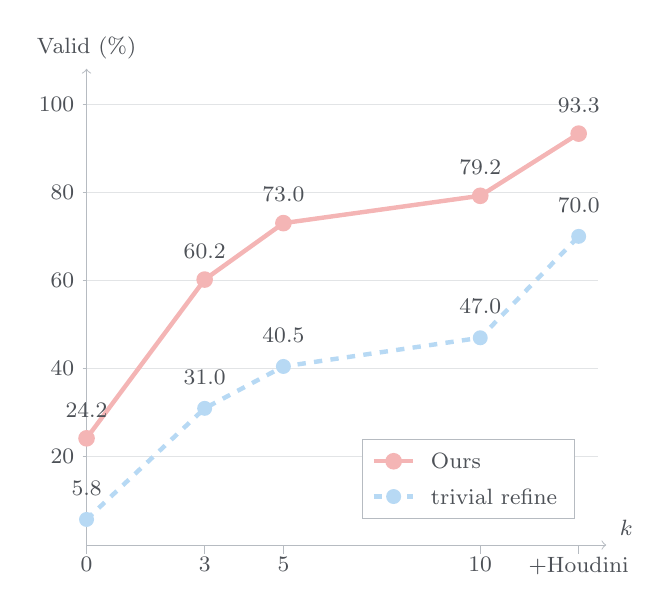
\begin{tikzpicture}[x=0.50cm,y=0.056cm,font=\footnotesize,every node/.style={text=figgraytext}]
  % Ours: full \toolname\ refine pipeline (SE-driven context, structured prompts,
  % rollback, ACSL fixer); trivial: minimal "fix-it" prompt, no rollback,
  % no ACSL fixer, no SE context. Both run with refine budget 10 + final Houdini.
  \def\za{24.2}  \def\zb{60.2}  \def\zc{73.0}  \def\zd{79.2}  \def\ze{93.3}
  \def\ta{5.8}   \def\tb{31.0}  \def\tc{40.5}  \def\td{47.0}  \def\te{70.0}
  \def\xH{12.5}
  % horizontal gridlines (faint)
  \foreach \y in {0,20,40,60,80,100} {
    \draw[figgrid] (0,\y) -- (\xH+0.5,\y);
  }
  % axes
  \draw[->,figaxis] (0,0) -- (\xH+0.7,0);
  \draw[->,figaxis] (0,0) -- (0,108);
  \node[anchor=west] at (\xH+0.8,4) {$k$};
  \node[anchor=south] at (0,108) {Valid (\%)};
  % y ticks (skip "0" to avoid colliding with the x=0 tick label)
  \foreach \y in {20,40,60,80,100} {
    \draw[figaxis] (-0.1,\y) -- (0,\y) node[left,xshift=-1pt] {\y};
  }
  % x ticks
  \foreach \x/\lab in {0/0,3/3,5/5,10/10,\xH/{+Houdini}} {
    \draw[figaxis] (\x,-2) -- (\x,0) node[below,yshift=-1pt] {\lab};
  }
  % Ours curve
  \draw[figcontractstroke,ultra thick] (0,\za) -- (3,\zb) -- (5,\zc) -- (10,\zd) -- (\xH,\ze);
  \foreach \x/\y in {0/\za,3/\zb,5/\zc,10/\zd,\xH/\ze} {
    \fill[figcontractstroke] (\x,\y) circle (2.6pt);
    \draw[figcontractstroke,line width=0.8pt] (\x,\y) circle (2.6pt);
    \node[anchor=south] at (\x,\y+2.6) {\y};
  }
  % trivial refine curve
  \draw[figloopstroke,ultra thick,dashed] (0,\ta) -- (3,\tb) -- (5,\tc) -- (10,\td) -- (\xH,\te);
  % all trivial labels above each point with consistent offset
  \foreach \x/\y in {0/\ta,3/\tb,5/\tc,10/\td,\xH/\te} {
    \fill[figloopstroke] (\x,\y) circle (2.3pt);
    \draw[figloopstroke,line width=0.8pt] (\x,\y) circle (2.3pt);
    \node[anchor=south] at (\x,\y+3.2) {\y};
  }
  % legend (lower-right, framed)
  \draw[figaxis,fill=white] (7.0,6) rectangle (12.4,24);
  \draw[figcontractstroke,ultra thick] (7.3,19) -- (8.3,19);
  \fill[figcontractstroke] (7.8,19) circle (2.6pt);
  \draw[figcontractstroke,line width=0.8pt] (7.8,19) circle (2.6pt);
  \node[anchor=west] at (8.5,19) {Ours};
  \draw[figloopstroke,ultra thick,dashed] (7.3,11) -- (8.3,11);
  \fill[figloopstroke] (7.8,11) circle (2.3pt);
  \draw[figloopstroke,line width=0.8pt] (7.8,11) circle (2.3pt);
  \node[anchor=west] at (8.5,11) {trivial refine};
\end{tikzpicture}
\caption{Cumulative \emph{Valid} rate on gpt-5.4-mini over 400 cases as the refinement budget \(k\) increases, for the full \toolname\ pipeline (\emph{Ours}) versus a \emph{trivial refine} baseline.}

\label{fig:refine-ablation}
\end{figure}

\section{Full Pass@k Benchmark Results}
\label{app:rq2-full}

Table~\ref{tab:performance_rates_model_full} supplements Table~\ref{tab:performance_rates_model} (Section~\ref{sec:experiments}) with the complete Pass@1/3/5 results per benchmark and model.

\begin{table*}[t]
\centering
\caption{Specification generation performance under Pass@1, Pass@3, and Pass@5 (complete table).}
\label{tab:performance_rates_model_full}

\setlength{\tabcolsep}{2pt}
\begin{adjustbox}{max width=\textwidth}
\begin{tabular}{cc ccc ccc ccc}
\toprule
\multirow{2}{*}{\textbf{Benchmark}} & \multirow{2}{*}{\textbf{Model}}
& \multicolumn{3}{c}{\textbf{Pass@1 (\%)}}
& \multicolumn{3}{c}{\textbf{Pass@3 (\%)}}
& \multicolumn{3}{c}{\textbf{Pass@5 (\%)}} \\
\cmidrule(lr){3-5} \cmidrule(lr){6-8} \cmidrule(lr){9-11}
& & \textbf{Syn.} & \textbf{Val.} & \textbf{Acc.}
& \textbf{Syn.} & \textbf{Val.} & \textbf{Acc.}
& \textbf{Syn.} & \textbf{Val.} & \textbf{Acc.} \\
\midrule

\multirow{4}{*}{\textbf{SyGuS}}
 & GPT-4o-mini & 90.98 & 87.97 & 78.20 & 97.74 & 95.49 & 88.72 & 98.50 & 96.99 & 90.23 \\
 & GPT-3.5-turbo & 93.23 & 88.72 & 84.21 & 97.74 & 97.74 & 92.48 & 98.50 & 98.50 & 93.23 \\
 & GPT-4o & 98.50 & 98.50 & 93.98 & 99.25 & 99.25 & 99.25 & 99.25 & 99.25 & 99.25 \\
 & Claude 3.7 Sonnet & 100.00 & 100.00 & 99.25 & 100.00 & 100.00 & 99.25 & 100.00 & 100.00 & 99.25 \\
    \midrule

\multirow{4}{*}{\textbf{OOPSLA}}
 & GPT-4o-mini & 80.43 & 65.22 & 32.61 & 89.13 & 86.96 & 43.48 & 89.13 & 86.96 & 47.83 \\
 & GPT-3.5-turbo & 82.61 & 54.35 & 41.30 & 86.96 & 65.22 & 45.65 & 86.96 & 67.39 & 47.83 \\
 & GPT-4o & 91.30 & 69.57 & 60.87 & 95.65 & 76.09 & 73.91 & 100.00 & 82.61 & 76.09 \\
 & Claude 3.7 Sonnet & 93.48 & 69.67 & 63.04 & 97.83 & 80.43 & 76.09 & 97.83 & 93.57 & 86.96 \\
\midrule

\multirow{4}{*}{\textbf{SV-COMP}}
 & GPT-4o-mini & 61.90 & 61.90 & 28.57 & 80.95 & 80.95 & 42.86 & 85.71 & 80.95 & 57.14 \\
 & GPT-3.5-turbo & 95.24 & 90.48 & 66.67 & 95.24 & 90.48 & 66.67 & 95.24 & 90.48 & 66.67 \\
 & GPT-4o & 90.48 & 90.48 & 52.38 & 100.00 & 100.00 & 71.43 & 100.00 & 100.00 & 76.19 \\
 & Claude 3.7 Sonnet & 100.00 & 100.00 & 71.43 & 100.00 & 100.00 & 71.43 & 100.00 & 100.00 & 76.19 \\
\midrule

\multirow{4}{*}{\textbf{NLA}}
 & GPT-4o-mini & 90.00 & 83.33 & 76.67 & 90.00 & 83.33 & 76.67 & 90.00 & 83.33 & 76.67 \\
 & GPT-3.5-turbo & 76.67 & 70.00 & 50.00 & 80.00 & 80.00 & 56.67 & 80.00 & 80.00 & 56.67 \\
& GPT-4o & 93.33 & 90.00 & 83.33 & 96.67 & 96.67 & 86.67 & 96.67 & 96.67 & 86.67 \\
& Claude 3.7 Sonnet & 96.67 & 96.67 & 86.67 & 96.67 & 96.67 & 86.67 & 96.67 & 96.67 & 86.67 \\
\midrule

\multirow{4}{*}{\textbf{numer-S}}
 & GPT-4o-mini & 95.00 & 90.00 & 72.50 & 100.00 & 95.00 & 75.00 & 100.00 & 95.00 & 75.00 \\
 & GPT-3.5-turbo & 92.50 & 85.00 & 62.50 & 95.00 & 90.00 & 65.00 & 95.00 & 92.50 & 67.50 \\
 & GPT-4o & 100.00 & 100.00 & 82.50 & 100.00 & 100.00 & 82.50 & 100.00 & 100.00 & 82.50 \\
 & Claude 3.7 Sonnet & 100.00 & 97.50 & 85.00 & 100.00 & 100.00 & 85.00 & 100.00 & 100.00 & 85.00 \\
\midrule

\multirow{4}{*}{\textbf{Frama-C}}
 & GPT-4o-mini & 54.90 & 49.02 & 47.06 & 62.75 & 50.98 & 49.02 & 64.71 & 50.98 & 49.02 \\
 & GPT-3.5-turbo & 77.08 & 60.42 & 52.08 & 83.33 & 62.50 & 54.17 & 83.33 & 62.50 & 54.17 \\
 & GPT-4o & 82.35 & 72.55 & 66.67 & 86.27 & 76.47 & 70.59 & 86.27 & 78.43 & 72.55 \\
 & Claude 3.7 Sonnet & 86.27 & 78.43 & 72.55 & 92.16 & 82.35 & 76.47 & 92.16 & 84.31 & 76.47 \\
\midrule

\multirow{4}{*}{\textbf{pIp}}
 & GPT-4o-mini & 90.00 & 87.50 & 65.00 & 92.50 & 92.50 & 72.50 & 92.50 & 92.50 & 75.00 \\
 & GPT-3.5-turbo & 84.00 & 76.00 & 66.00 & 88.00 & 78.00 & 72.00 & 88.00 & 78.00 & 76.00 \\
 & GPT-4o & 94.00 & 78.00 & 64.00 & 94.00 & 78.00 & 76.00 & 94.00 & 78.00 & 78.00 \\
 & Claude 3.7 Sonnet & 100.00 & 88.00 & 82.00 & 100.00 & 90.00 & 88.00 & 100.00 & 92.00 & 88.00 \\
\midrule

\multirow{4}{*}{\textbf{list-S}}
 & GPT-4o-mini & 62.50 & 41.67 & 33.33 & 75.00 & 45.83 & 41.67 & 79.17 & 54.17 & 45.83 \\
 & GPT-3.5-turbo & 70.83 & 20.83 & 8.33 & 79.17 & 25.00 & 16.67 & 79.17 & 25.00 & 16.67 \\
 & GPT-4o & 70.83 & 62.50 & 54.17 & 87.50 & 83.33 & 75.00 & 91.67 & 87.50 & 79.17 \\
 & Claude 3.7 Sonnet & 95.83 & 83.33 & 75.00 & 100.00 & 100.00 & 95.83 & 100.00 & 100.00 & 95.83 \\
\bottomrule
\end{tabular}
\end{adjustbox}
\end{table*}

\section{{Translation Detail}}
\label{app:benchmark-translation}

{We used GPT-5.4 to translate the 250 FormalBench and 59 SpecGenBench Java programs into C; the other 91 SV-COMP cases are native C. For each Java case, the model was asked to preserve the target method's branches, loops, assignments, and returns while adapting its types and memory operations to C. We removed JML annotations and goal assertions and renamed the target function to \texttt{foo} followed by its case ID. Programs that could not be translated into the supported C fragment and compiled were excluded; for example, SpecGenBench's \texttt{ConvertToTitle} uses Java \texttt{StringBuffer.append} and \texttt{reverse} and was not included. All 400 selected C programs pass GCC C11 compilation: 309 translated programs and 91 native-C programs.}

{In the resulting programs, Java \texttt{int}, \texttt{long}, and \texttt{boolean} are represented by C \texttt{int}, \texttt{long long}, and 0/1-valued \texttt{int}. An array parameter \texttt{int[] a} becomes \texttt{int *a, int a\_len}; \texttt{a.length} becomes \texttt{a\_len}, and array lengths are passed through calls. A local \texttt{new int[n]} becomes a C allocation with a stored length. Constants such as \texttt{Integer.MIN\_VALUE} and the few string operations are adapted to their C counterparts.}

{Compilation checks syntax, not full semantic equivalence. Cross-language comparisons are restricted to normal executions with valid memory accesses, successful allocation, and no signed overflow.}

{We also checked translation behavior by differential execution on all 309 Java/C pairs. The check covered 4,325 comparable executions using deterministic edge-case and seeded pseudorandom inputs, and compared the return value and any modified integer-array arguments. The Java programs were compiled for Java 8, and the C programs were compiled with GCC C11 and undefined-behavior checks. Of these executions, 4,323 produced matching observations; the other two triggered C undefined behavior in the same program. Thus, 308 of 309 pairs showed no discrepancy on their tested inputs, while one pair exposed a cross-language semantic difference.}

{In that pair, case 112, input \texttt{'0'} makes the expression \texttt{1 << (c - 'a')} shift by a negative count in C, whereas Java defines the shift and returns 1. This discrepancy is outside the common defined-behavior domain, but it shows why compilation and finite-input agreement cannot establish unrestricted Java/C equivalence.}

\section{{Specification Strength Comparison}}
\label{app:strength}

{This appendix collects the complete material for the dimension-wise specification-strength study of Section~\ref{subsec:rq6-strength}: the comparison protocol, the judge configuration and prompts, the full pairwise results for both baselines including the cross-language comparison against \specgen\ (Java/JML), and the A/B-order audit of the LLM judge.}

\subsection{{Comparison protocol}}
\label{app:strength-protocol}

{Validity certifies that a specification is discharged by its verifier, but it does not rank how informative it is. We therefore compare accepted input domains (preconditions), normal-return guarantees (postconditions), and predicates at corresponding loop points (loop invariants) independently. Each dimension uses a separate judge prompt and API call. Preconditions are classified by set inclusion between their accepted input domains; postconditions are compared by bidirectional implication over the common input domain; and invariants are compared at corresponding loop points. Thus, the two directional columns in Table~\ref{tab:strength_summary_full} mean more permissive for preconditions and logically stronger for postconditions and invariants. We do not aggregate them into an overall contract ranking. A missing precondition or postcondition denotes \texttt{true}. Expert review corrected 32 judge verdicts, shown as transitions in Table~\ref{tab:strength_summary_full}; any implication that cannot be established is included in Incomp.}

\subsection{{Judge configuration}}
\label{app:judge-config}

{We used GPT-5.4 with a 2,048-token output limit, no input truncation, and the provider-default temperature, top-$p$, and reasoning effort. Each precondition, postcondition, and loop-invariant comparison used a separate API call and the corresponding prompt in Section~\ref{app:prompt-strength-judge}. The expert review was conducted by two master's-level researchers with formal-verification backgrounds.}

\subsection{{Pairwise specification strength judges}}
\label{app:prompt-strength-judge}

{Fig.~\ref{fig:prompt-judge} gives the three independent judge prompts used for the pairwise comparisons reported in Section~\ref{subsec:rq6-strength} and Table~\ref{tab:strength_summary_full}. Each invocation receives only the target function's annotation blocks relevant to that dimension; the complete prompt text and structured responses are included in the artifact.}

\par\medskip\noindent
\begin{minipage}[t]{\columnwidth}
\begin{tcolorbox}[promptboxcompact, title={\textcolor{white}{Precondition judge}}, width=\linewidth]
\begin{lstlisting}[style=PromptInnerCompact]
[System]
Compare only accepted input domains. A missing
precondition means true. Report which predicate is
WEAKER, i.e., which one accepts more inputs.
Do not compare postconditions or invariants.

[User]
Evaluate independently:
  B_to_A: P_B implies P_A
  A_to_B: P_A implies P_B
B_to_A only => A_accepts_more
A_to_B only => B_accepts_more
both => equivalent
neither/unknown => incomparable
Return both directions, the relation, and a concise
implication-based reason as strict JSON.
\end{lstlisting}
\end{tcolorbox}
\end{minipage}\par\medskip\noindent
\begin{minipage}[t]{\columnwidth}
\begin{tcolorbox}[promptboxcompact, title={\textcolor{white}{Postcondition judge}}, width=\linewidth]
\begin{lstlisting}[style=PromptInnerCompact]
[System]
Compare only normal-return guarantees on the common
accepted input domain. Missing preconditions or
postconditions mean true. Ignore invariant content.

[User]
Let D = P_A AND P_B. Evaluate independently:
  A_to_B: D AND Q_A implies Q_B
  B_to_A: D AND Q_B implies Q_A
A_to_B only => A_guarantees_more
B_to_A only => B_guarantees_more
both => equivalent
neither/unknown => incomparable
Do not reward a wider input domain or infer an
unstated guarantee from the body. Return both
implication directions, relation, and reason as JSON.
\end{lstlisting}
\end{tcolorbox}
\end{minipage}\par\medskip\noindent
\begin{minipage}[t]{\columnwidth}
\begin{tcolorbox}[promptboxcompact, title={\textcolor{white}{Loop-invariant judge}}, width=\linewidth]
\begin{lstlisting}[style=PromptInnerCompact]
[System]
Compare only explicit loop invariants at corresponding
program points. Ignore function contracts.

[User]
At each point, conjoin that side's invariants.
Evaluate independently at every point:
  A_to_B: I_A implies I_B
  B_to_A: I_B implies I_A
A_to_B only => A_invariants_stronger
B_to_A only => B_invariants_stronger
both everywhere => equivalent
neither/unknown => incomparable
Do not merge different loop points or infer reachable
states from bodies. Return both implication directions,
relation, and a concise decisive reason as JSON.
\end{lstlisting}
\end{tcolorbox}
\end{minipage}
\begin{figure}[H]
\caption{{Independent strength-judge prompts used before expert review. A and B denote two anonymized specifications; tool identities are not disclosed to the judge.}}
\label{fig:prompt-judge}
\end{figure}

\subsection{{Full pairwise results}}
\label{app:strength-results}

{Table~\ref{tab:strength_summary_full} reports the complete dimension-wise results on the both-valid sets for both baselines. The \autospec\ (C/ACSL) rows and the Frama-C/WP cross-check are discussed in Section~\ref{subsec:rq6-strength}; the remainder of this subsection analyzes the cross-language comparison against \specgen\ (Java/JML).}

\begin{table*}[t]
\centering
\caption{{Pairwise dimension-wise relations on both-valid sets, reported as LLM judge $\rightarrow$ judge + expert review. Invariant comparisons include only pairs for which both tools produced loop invariants.}}
\label{tab:strength_summary_full}
\setlength{\tabcolsep}{5pt}
\begin{adjustbox}{max width=\textwidth}
\begin{tabular}{llrrrrr}
\toprule
\textbf{Baseline} & \textbf{Dimension} & \textbf{Evaluated} & {\textbf{\toolname\ side}} & {\textbf{Baseline side}} & \textbf{Equal} & \textbf{Incomp.} \\
\midrule
\multirow{3}{*}{\autospec\ (C/ACSL)}
 & {Preconditions} & {698} & {96$\rightarrow$96} & {290$\rightarrow$290} & {311$\rightarrow$311} & {1$\rightarrow$1} \\
 & {Postconditions} & {698} & {342$\rightarrow$342} & {18$\rightarrow$18} & {320$\rightarrow$320} & {18$\rightarrow$18} \\
 & {Loop invariants} & {540} & {120$\rightarrow$120} & {50$\rightarrow$52} & {5$\rightarrow$5} & {365$\rightarrow$363} \\
\midrule
\multirow{3}{*}{\specgen\ (Java/JML)}
 & {Preconditions} & {673} & {161$\rightarrow$164} & {178$\rightarrow$174} & {221$\rightarrow$222} & {113$\rightarrow$113} \\
 & {Postconditions} & {673} & {102$\rightarrow$100} & {246$\rightarrow$244} & {218$\rightarrow$220} & {107$\rightarrow$109} \\
 & {Loop invariants} & {473} & {183$\rightarrow$183} & {9$\rightarrow$9} & {2$\rightarrow$2} & {279$\rightarrow$279} \\
\bottomrule
\end{tabular}
\end{adjustbox}
\end{table*}

{Against \specgen, \toolname\ leads on loop invariants but \specgen\ leads on postconditions. One contributing factor is the difference between the two verification settings: the Java/JML and OpenJML stack supports high-level functional contracts without the pointer-validity and buffer-related obligations required by ACSL and Frama-C/WP. In the C setting, these additional memory-model obligations can make some postconditions difficult for Frama-C/WP to discharge, so \toolname's verification-driven pipeline may retain fewer postconditions when the corresponding proof obligations cannot be discharged within the allotted budget. The comparison therefore reflects both specification generation and differences in the underlying language and verification stacks.}

{We omit a WP cross-check for \specgen\ because translating Java/JML reference and array semantics into ACSL would confound the comparison.}



\subsection{{Position-bias audit (A/B order)}}
\label{app:judge-audit}

{The primary run placed the baseline in A and \toolname\ in B. To test order sensitivity, we repeated every judge decision with \toolname\ in A and the baseline in B, then mapped the output back to the original tool orientation. Table~\ref{tab:judge-position-audit} compares the raw judge results before expert correction. Pairs with no substantive predicate on either side are deterministically equal and are included in the reported agreement. The principal AutoSpec trends remain stable under the swapped order. For SpecGen, the postcondition and invariant directions also persist, while the precondition direction changes, indicating greater order sensitivity for this cross-language comparison.}

\begin{table}[H]
\centering
\caption{{A/B-order audit of the LLM judge. Outcome tuples are \toolname/baseline/equal/incomparable.}}
\label{tab:judge-position-audit}
\setlength{\tabcolsep}{2pt}
\renewcommand{\arraystretch}{0.9}
\begin{tabular}{lrrrr}
\toprule
{\textbf{Dimension}} & {\textbf{Pairs}} & {\textbf{Agreement}} & {\textbf{Primary}} & {\textbf{Swapped}} \\
\midrule
\multicolumn{5}{l}{{\autospec\ (C/ACSL)}} \\
{Preconditions} & {698} & {695 (99.6\%)} & {96/290/311/1} & {99/288/310/1} \\
{Postconditions} & {698} & {672 (96.3\%)} & {342/18/320/18} & {349/11/325/13} \\
{Loop invariants} & {540} & {435 (80.6\%)} & {120/50/5/365} & {160/49/5/326} \\
\midrule
\multicolumn{5}{l}{{\specgen\ (Java/JML)}} \\
{Preconditions} & {673} & {546 (81.1\%)} & {161/178/221/113} & {200/86/232/155} \\
{Postconditions} & {673} & {518 (77.0\%)} & {102/246/218/107} & {141/203/217/112} \\
{Loop invariants} & {473} & {382 (80.8\%)} & {183/9/2/279} & {198/3/1/271} \\
\bottomrule
\end{tabular}
\end{table}

\section{Case Studies}
\label{app:cases}
\suppressfloats[t]

This appendix presents ten case studies that show, on concrete programs, what symbolic execution contributes to generated specifications. Across all cases, \toolname\ reuses the same local symbolic context and template-routing signals, so each case emphasizes a distinct role of that context rather than repeating the full mechanism. Table~\ref{tab:case-study-map} summarizes the cases, which cover loop phases, C aliasing, recursive heap shapes, RTE safety versus functional specification, an industrial pipeline, inductive helpers, signed arithmetic, recursion, and matrix multiplication. In the figures below, ACSL annotations enclosed by $/*@\cdots */$ are generated by \toolname\ and then retained after verification or pruning.

%Note that in all figures, the black boxes highlight the portions generated by the LLM, while the remaining elements are automatically derived through symbolic execution.

\begin{table}[H]
  \centering
  \caption{Organization of the case studies.}
  \label{tab:case-study-map}
  \begin{adjustbox}{max width=\linewidth}
  \begin{tabular}{ll}
    \toprule
    \textbf{Case} & \textbf{Main lesson} \\
    \midrule
    1. SyGuS loop & Phase-split invariant from weak goals \\
    2. TripleAbsMax & Path-complete C/ACSL postconditions \\
    3. Linked list & Shape-predicate routing \\
    4. Linear search & RTE-safety vs.\ functional specification \\
    5. Industrial pipeline & Scale and verifier boundary \\
    6. Factorial & Guarded inductive helper \\
    7. GCD & Recursive summary with a simple measure \\
    8. MulLoop & Sign-sensitive loop invariant \\
    9. Ackermann & ACSL/SMT recursion boundary \\
    10. Matrix multiply & Nested loops; verifier/SMT-timeout boundary \\
    \bottomrule
  \end{tabular}%
  \end{adjustbox}
\end{table}

\subsection{Case 1: Phase-Split Invariant from a Weak Goal}

\begin{figure}[!t]
    \centering
    \begin{tcolorbox}[casebox, title={Case 1: symbolic state exposes loop phases}]
\begin{lstlisting}[style=caseinnerstyle]
int unknown();

/*@ requires n > 0; */
void SyGuS38(int n) {
  int c = 0;

  /*@
    loop invariant ((c == 0)&&(n == \at(n,Pre))) || (1 <= c <= n) ;
    loop invariant n == \at(n,Pre);
    loop assigns c ;
  */
  while (unknown()) {
    if(c == n) {
      c = 1;
    }
    else {
      c = c + 1;
    }
  }

  /*@ assert (c == n) ==> (c >= 0); */
}
\end{lstlisting}
    \end{tcolorbox}
    \caption{Case 1 (SyGuS-38): a nondeterministic loop whose phase structure is exposed by symbolic execution.}
    \label{fig:case1}
\end{figure}

Fig.~\ref{fig:case1} isolates the benefit of symbolic execution when the assertion is too weak to guide invariant synthesis. The goal $(c = n) \Rightarrow (c \ge 0)$ can be proved by many uninformative invariants; what matters here is the loop's phase structure.

At the loop boundary, symbolic execution separates the unentered state (\texttt{c == 0}) from the inductive region (\texttt{1 <= c <= n}) and records that \texttt{n} is stable. The disjunctive template instantiates exactly that split, yielding an invariant that describes the loop behavior rather than merely satisfying the final assertion.

\subsection{Case 2: Path-Complete Postconditions {for Pointer-Manipulating Code}}

\begin{figure}[!t]
    \centering
    \begin{tcolorbox}[casebox, title={\textcolor{white}{Case 2: path-complete postconditions for pointer-manipulating code}}, width=\linewidth]
\begin{lstlisting}[style=casecompactinnerstyle]
typedef struct __TripleAbsMax
{
  int abs[3];
  int tmax;
  int* ret;
} TripleAbsMax;

/*@
  requires \valid(pIp);
  requires \valid(pIp->abs+(0..2)) ;
  requires \valid(pIp->ret);
  requires \separated(pIp, pIp->ret);

  ensures pIp->ret == \old(pIp->ret);
  ensures -pIp->abs[2] <= pIp->abs[1] && pIp->abs[0] <= pIp->abs[1] && pIp->abs[2] < 0 && pIp->abs[1] >= 0
  && pIp->abs[0] >= 0 ==> pIp->tmax == pIp->abs[1] && *\old(pIp->ret) == pIp->abs[1];
  ... all 32 paths

  assigns pIp->tmax, *(pIp->ret);
*/
void TripleAbsMaxFun(TripleAbsMax *pIp)
{
  int absfx1 = pIp->abs[0];
  int absfy2 = pIp->abs[1];
  int absfz3 = pIp->abs[2];

  if (pIp->abs[0] < 0){  absfx1 = -pIp->abs[0];}

  if (pIp->abs[1] < 0){  absfy2 = -pIp->abs[1];}

  if (pIp->abs[2] < 0){  absfz3 = -pIp->abs[2];}

  if (absfx1 > absfy2){  pIp->tmax = absfx1;}
  else{ pIp->tmax = absfy2; }

  if (absfz3 > pIp->tmax){pIp->tmax = absfz3;}

  *(pIp->ret) = pIp->tmax;
}

/*@
  requires \valid(pIp);
  requires \valid(pIp->abs+(0..2));
  requires \valid(pIp->ret);
  requires \separated(pIp, pIp->ret);
*/
void main1(TripleAbsMax *pIp)
{
  pIp -> abs[0] = 1;
  pIp -> abs[1] = 2;
  pIp -> abs[2] = -3;

  TripleAbsMaxFun(pIp);

  /*@ assert pIp -> tmax == 3; */
}
\end{lstlisting}
    \end{tcolorbox}
    \caption{Case 2 (TripleAbsMax): {a loop-free program with 32 feasible paths under the precondition shown.}}
    \label{fig:case3}
\end{figure}

Fig.~\ref{fig:case3}, from our \textbf{pIp} benchmark, is the main C-specific case. The function computes the maximum absolute value of three struct-stored integers and writes it both to \texttt{pIp->tmax} and through \texttt{pIp->ret}.

{Starting from the default precondition, including \texttt{\textbackslash separated(pIp, pIp->ret)}, symbolic execution derives the guarded postconditions for the feasible paths.}
\subsection{Case 3: Shape-Predicate Routing for Linked Structures}

\begin{figure}[!t]
    \centering
    \begin{tcolorbox}[casebox, title={Case 3: route-selected shape predicates}]
\begin{lstlisting}[style=caseinnerstyle]
struct SLL {
    struct SLL *tail;
    int head;
};

/*@
  predicate lseg{L}(struct SLL* x, struct SLL* y) =
    x == y || (x != y && \valid(x) && \separated(x, y) && lseg{L}(x->tail, y));
*/

/*@ predicate listrep(struct SLL* head) = lseg(head, \null); */

/*@
  logic integer list_length{L}(struct SLL* x) =
    (x == \null) ? 0 : 1 + list_length{L}(x->tail);
*/

/*@
  requires listrep(l);
  requires \valid_read(&data);
  assigns \nothing;
  ensures listrep(l);
  ensures \result == l;
*/
struct SLL * main1(struct SLL *l, int data)
{
    struct SLL *p;
    p = l;

    /*@
      loop invariant listrep(p);
      loop invariant listrep(l);
      loop invariant lseg(l, p);
      loop invariant data == \at(data,Pre);
      loop invariant l == \at(l,Pre);
      loop invariant list_length(l) >= list_length(p);
      loop assigns p;
    */
    while (p) {
      if (p->head == data) {
        /*@ assert data == \at(data,Pre); */
        /*@ assert l == \at(l,Pre); */
        return l;
      }
      p = p->tail;
    }

    return l;
}
\end{lstlisting}
    \end{tcolorbox}
    \caption{Case 3 (linked-list traversal): a recursive data-structure program with shape predicates.}
    \label{fig:case4}
\end{figure}

Fig.~\ref{fig:case4} illustrates template routing for a linked-list traversal. The loop walks a singly linked list and returns the original head pointer, so ACSL needs an explicit heap-shape abstraction instead of only arithmetic facts.

Symbolic execution identifies \texttt{p} as the advancing list pointer and records the local update facts, while the static route recognizes the recursive type and field-access pattern. That route selects the recursive-shape template, which supplies \texttt{lseg}, \texttt{listrep}, and \texttt{list\_length}; the loop template then connects the original head to the current suffix through \texttt{lseg(l, p)}. The program-structure route supplies shape predicates, and symbolic cursor facts anchor them to this traversal.

\subsection{Case 4: RTE Safety vs. Functional Specification}
\label{app:case-search}

We run \toolname\ on the linear search source from Fig.~3 of Preguss~\cite{Wang2025ATO} to illustrate the difference between RTE-guided safety specifications and goal-independent functional specifications. \toolname\ records potential RTE reports as warnings during Frama-C validation. An RTE can still block QCP symbolic execution: the default flattened-memory precondition provides modeled validity, bounds, and separation facts, while arithmetic and pointer-related RTEs may require stronger preconditions. Refinement can add those preconditions when the failure is visible.

\begin{figure}[!t]
  \centering
  \begin{tcolorbox}[casebox, title={Preguss: RTE-guided safety specification}, width=0.96\linewidth]
\begin{lstlisting}[style=casecompactinnerstyle]
/*@ requires \valid_read(arr+(0..len-1));
    assigns \nothing; */
int * search(int * arr, int len, int val) {
    int i = 0;
    /*@ loop assigns i; */
    while (i < len) { ... }
}
\end{lstlisting}
  \end{tcolorbox}
  \vspace{1.4ex}

  \begin{tcolorbox}[casebox, title={\toolname: verifier-checked prefix-search specification}, width=0.96\linewidth]
\begin{lstlisting}[style=casecompactinnerstyle]
/*@ logic integer count_eq{L}(int* a, integer lo,
      integer hi, integer v) =
      lo >= hi ? 0 : count_eq(a, lo, hi - 1, v)
                   + (a[hi - 1] == v ? 1 : 0); */
/*@ requires \valid(arr + (0 .. len - 1));
    requires len >= 0;
    ensures \forall integer k; 0 <= k < len ==>
              arr[k] == \at(arr[k], Pre);
    ensures \result == \null ==>
              count_eq(arr, 0, len, val) == 0;
    ensures \result != \null ==>
              count_eq(arr, 0, \result - arr, val) == 0
              && *\result == val;
    assigns \nothing; */
int * search(int * arr, int len, int val) {
    int i = 0;
    /*@ loop invariant 0 <= i <= len;
        loop invariant \forall integer k;
            0 <= k < len ==> arr[k] == \at(arr[k], Pre);
        loop invariant count_eq(arr, 0, i, val) == 0;
        loop assigns i; loop variant len - i; */
    while (i < len) {
        if (arr[i] == val) return arr + i;
        i = i + 1;
    }
    return (int *)0;
}
\end{lstlisting}
  \end{tcolorbox}
  \caption{Case 4 (linear search). Preguss verifies memory-access safety; \toolname\ also captures the prefix-search property and returned-pointer consequence.}
  \label{fig:case7}
\end{figure}

Fig.~\ref{fig:case7} shows the difference in target. Preguss emits the memory-safety precondition needed to discharge \texttt{arr[i]} accesses. \toolname\ instead routes the loop to a count-occurrences helper and records both return cases: null means \texttt{val} is absent, and non-null means the returned pointer dereferences to \texttt{val} with no earlier occurrence. This illustrates why RTE-safety synthesis of Preguss~\cite{Wang2025ATO} and our functional specification synthesis should not be read as identical tasks.

\subsection{Case 5: Industrial Pipeline Stress Test}
\label{subsec:case9-ip}

\begin{figure*}[!t]
    \centering
    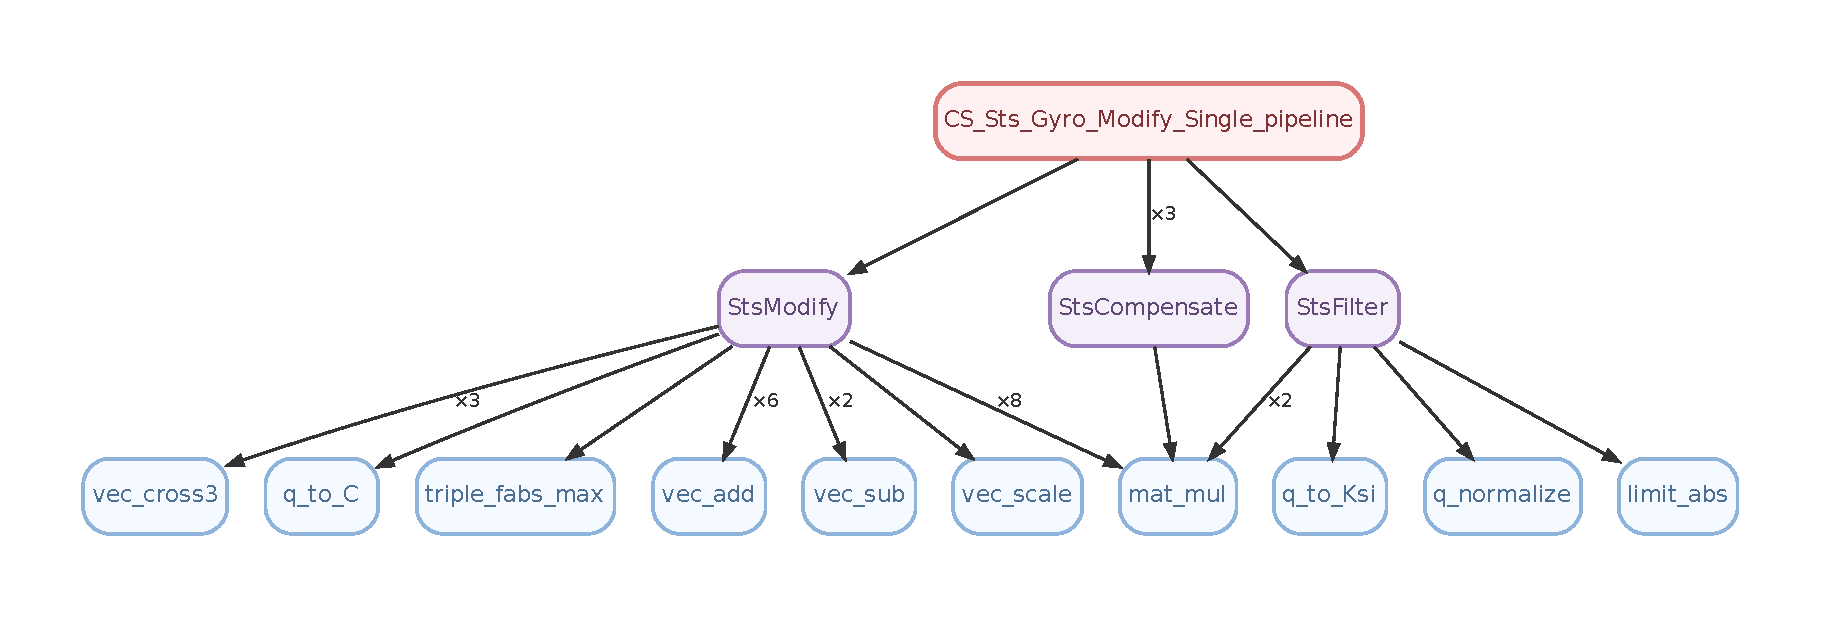
\includegraphics[width=0.95\textwidth]{images/ip_callgraph.pdf}
    \caption{Call graph of the single-star-sensor filter-update pipeline. Edge labels show call multiplicity; unlabeled edges are $\times 1$.}
    \label{fig:case9-callgraph}
\end{figure*}

\smallskip
\noindent\textbf{Program structure.}
We applied \toolname\ to a 225-line C transcription of an industrial single-star-sensor Kalman-update pipeline. The translation unit contains 14 functions, 33 call sites, and 8 loops; the entry delegates to three pipeline stages, which in turn call ten numeric and quaternion helpers (Fig.~\ref{fig:case9-callgraph}). This case is included to show the scale boundary, not another single function invariant pattern.

\smallskip
\noindent\textbf{What \toolname\ produced.}
Driven by \texttt{gpt-5.4-mini} at maximum reasoning effort (\texttt{reasoning\_effort=high}) in the goal-independent configuration, {\toolname\ completed specification generation for 13 of the 14 functions.} The assembled file contains 198 ACSL clauses, and Frama-C/WP discharges 601 of 625 verification conditions ($96.2\%$) at a 30\,s per-goal timeout. Table~\ref{tab:case9-wp} shows that increasing the timeout from 5\,s to 30\,s recovers only one additional goal, so the residual failures reflect hard proof obligations rather than transient budget noise.

{To complement the proof-discharge rate, we also manually audited the functional content of each accepted contract. We count a postcondition as functional only when it gives a non-vacuous relation between the output or return value and the inputs; \texttt{ensures \textbackslash true} receives no such credit. Ten functions have functional postconditions: \texttt{limit\_abs}, \texttt{q\_to\_C}, \texttt{q\_to\_Ksi}, \texttt{triple\_fabs\_max}, \texttt{vec\_cross3}, \texttt{vec\_scale}, \texttt{vec\_add}, \texttt{vec\_sub}, \texttt{StsCompensate}, and \texttt{StsFilter}. The other four lack a complete functional summary: \texttt{StsModify} provides only output bounds, \texttt{mat\_mul} has the vacuous \texttt{ensures \textbackslash true}, and the no-op helper \texttt{q\_normalize} and the top-level \texttt{CS\_Sts\_Gyro\_Modify\_Single\_pipeline} have no explicit accepted contract.}

\begin{table}[!t]
  \centering
  \caption{Frama-C/WP proof obligations for the aerospace pipeline.}
  \label{tab:case9-wp}
  \begin{tabular}{lrrr}
    \toprule
    & \multicolumn{3}{c}{\textbf{per-goal timeout}} \\
    \cmidrule(lr){2-4}
    \textbf{Disposition} & \textbf{5\,s} & \textbf{10\,s} & \textbf{30\,s} \\
    \midrule
    Total       & 625           & 625           & 625           \\
    Valid       & 600           & 601           & 601           \\
    Unknown     & 2             & 2             & 3             \\
    Timeout     & 23            & 22            & 21            \\
    \midrule
    Discharge rate & $96.0\%$ & $96.2\%$ & $96.2\%$ \\
    \bottomrule
  \end{tabular}
\end{table}

\smallskip
\noindent\textbf{Boundary exposed.}
{The functions with functional summaries are mostly arithmetic leaves whose semantics admit closed-form ACSL relations, such as \texttt{limit\_abs}, \texttt{vec\_cross3}, and \texttt{q\_to\_C}.} The hard cases are delegate functions and matrix-style loops: composing multi-stage callee summaries and expressing row-major matrix products require either user-provided logic summaries or proof automation beyond the current SMT-only backend. {Together, the $96.2\%$ discharge rate and contract audit characterize both verifier acceptance and functional coverage.} Concretely, the undischarged goals concentrate in the matrix-multiply leaf \texttt{mat\_mul} and its callers, exactly the triple-nested product dissected in Case~10 below, where the recursive \texttt{mat\_sum} over nonlinear indices makes Z3 time out and the accepted specification degrades to \texttt{ensures \textbackslash true}.

\Needspace*{10\baselineskip}
\subsection{Case 6: Guarded Inductive Helper for Factorial}
\label{app:case-factorial}

\begin{figure}[!b]
    \centering
    \begin{tcolorbox}[casebox, title={Case 6: guarded factorial helper}, width=\linewidth]
\begin{lstlisting}[style=casecompactinnerstyle]
int unknown();

/*@
  logic integer product(integer begin, integer end) =
    (end < begin) ? 1 : product(begin, end - 1) * end;
*/

/*@
  requires \true;
  assigns \nothing;
  ensures (n < 1) ==> \result == 1;
  ensures (n >= 1) ==> \result == product(1, n);
*/
int factorial9(int n) {
  int i = 1;
  int f = 1;

  /*@
    loop invariant (1 <= \at(n,Pre)) ==> (1 <= i <= n + 1);
    loop invariant (1 <= \at(n,Pre)) ==> (f == product(1, i - 1));
    loop invariant (!(1 <= \at(n,Pre))) ==> ((f == 1)&&(i == 1)&&(n == \at(n,Pre)));
    loop invariant n == \at(n,Pre);
    loop assigns f, i;
  */
  while (i <= n) {
    f = f * i;
    i = i + 1;
  }

  return f;
}

void goo9() {
  int t = factorial9(5);
  //@ assert t == 120;
}
\end{lstlisting}
    \end{tcolorbox}
    \caption{Case 6 (factorial): a guarded loop invariant with a recursive \texttt{product} helper.}
    \label{fig:case2}
\end{figure}

Fig.~\ref{fig:case2} complements the phase-split loop case (Case 1) above: the loop may be skipped when \texttt{n < 1}, and the entered region requires the inductive relation \texttt{f == product(1, i - 1)}. Symbolic execution provides the entered/unentered guard, while the static route selects the inductive-helper template that supplies the ACSL \texttt{product} definition used by both the invariant and the postcondition.

\Needspace*{10\baselineskip}
\subsection{Case 7: Recursive GCD Summary with a Simple Measure}
\label{app:case-gcd}

\begin{figure}[!b]
    \centering
    \begin{tcolorbox}[casebox, title={Case 7: recursive GCD summary}]
\begin{lstlisting}[style=casecompactinnerstyle]
/*@ 
  logic integer gcd_logic(integer a, integer b) =
    (a == 0) ? b :
    (b == 0) ? a :
    (a == b) ? a :
    (a > b) ? gcd_logic(a - b, b) :
               gcd_logic(a, b - a);
*/

/*@
requires \true;
decreases a + b;
assigns \nothing;
ensures \result == gcd_logic(a, b);
*/
int gcd(int a, int b) 
{
    if (a == 0)
       return b;

    if (b == 0)
       return a;

    if (a == b)
        return a;

    if (a > b)
        return gcd(a-b, b);
    return gcd(a, b-a);
}

int main2()
{
    int a = 98, b = 56;
    int c = gcd(a, b);
    //@ assert c == 14;
    return 0;
}
\end{lstlisting}
    \end{tcolorbox}
    \caption{Case 7 (GCD): a recursive logic summary with a single arithmetic termination measure.}
    \label{fig:case5}
\end{figure}

Fig.~\ref{fig:case5} shows the recursion case where the current workflow succeeds cleanly. When symbolic execution reaches a recursive call, \toolname\ switches to the recursion template, emits \texttt{gcd\_logic} branch-by-branch, and uses \texttt{decreases a + b}. This case is useful mainly as a contrast to the Ackermann case below: GCD needs only a single-measure descent and a single-unfold style of reasoning.

\Needspace*{10\baselineskip}
\subsection{Case 8: Signed Multiplication Loop}
\label{app:case-mulloop}

\begin{figure}[!b]
    \centering
    \begin{tcolorbox}[casebox, title={Case 8: signed multiplication loop}]
\begin{lstlisting}[style=casecompactinnerstyle]
int foo57(int a, int b);

/*@
  requires \true;
  assigns \nothing;
  ensures \result == a * b;
*/
int foo57(int a, int b) {
    int res = 0;
    if (b >= 0) {
        /*@
          loop invariant 0 <= i <= b;
          loop invariant res == i * a;
          loop assigns i, res;
          loop variant b - i;
        */
        for (int i = 0; i < b; i++) {
            res = res + a;
        }
    } else {
        /*@
          loop invariant 0 <= i <= -b;
          loop invariant res == -i * a;
          loop assigns i, res;
          loop variant -b - i;
        */
        for (int i = 0; i < -b; i++) {
            res = res - a;
        }
    }
    return res;
}
\end{lstlisting}
    \end{tcolorbox}
    \caption{Case 8 (MulLoop) from \textbf{SpecGenBench}.}
    \label{fig:case6}
\end{figure}

Fig.~\ref{fig:case6} computes $a \cdot b$ by addition or subtraction depending on the sign of \texttt{b}. The negative branch requires the asymmetric invariant \texttt{res == -i * a}; reusing the positive-branch form would make the functional postcondition fail. In our run, \toolname\ retains \texttt{ensures \textbackslash result == a * b} because the branch condition selects the correct invariant template.

\Needspace*{10\baselineskip}
\subsection{Case 9: Ackermann Recursion Beyond ACSL/SMT Automation}
\label{app:case-ackermann}

\begin{figure}[!b]
    \centering
    \begin{tcolorbox}[casebox, title={Case 9: Ackermann recursion boundary}]
\begin{lstlisting}[style=casecompactinnerstyle]
int foo1(int m, int n);

/*@
  logic integer ackermann(integer m, integer n) =
    (m == 0) ? n + 1 :
    (n == 0) ? ackermann(m - 1, 1) :
               ackermann(m - 1, ackermann(m, n - 1));
*/

/*@
  requires m >= 0 && n >= 0;
  decreases m * 1000 + n;
  assigns \nothing;
  ensures \result == ackermann(m, n);
*/
int foo1(int m, int n) {
    if (m == 0) {
        return n + 1;
    }
    if (n == 0) {
        return foo1(m - 1, 1);
    }
    return foo1(m - 1, foo1(m, n - 1));
}
\end{lstlisting}
    \end{tcolorbox}
    \caption{Case 9 (Ackermann). The candidate specification is syntactically clean but not discharged by Frama-C/WP under the current ACSL/SMT backend.}
    \label{fig:case8}
\end{figure}

Fig.~\ref{fig:case8} marks a boundary rather than a prompt failure. The generated helper follows the C branch structure, but Ackermann needs a lexicographic termination argument and nested induction that are not handled well by the current ACSL/SMT stack. A scalar \texttt{decreases m * 1000 + n} is not a sound substitute for the true lexicographic descent once \texttt{n} grows, and the functional postcondition would require proof support beyond the single-unfold reasoning that succeeds for GCD.

\Needspace*{10\baselineskip}
\subsection{Case 10: Matrix Multiplication Beyond Per-Loop Symbolic Context}
\label{app:case-matmul}

\begin{figure}[!b]
    \centering
    \begin{tcolorbox}[casebox, title={Case 10: matrix-multiplication proof boundary}, width=\linewidth]
\begin{lstlisting}[style=casecompactinnerstyle]
/*@
  logic integer mat_sum(int *A, int *B, integer ca_rb, integer cb,
                        integer i, integer j, integer k) =
    k <= 0 ? 0 :
    mat_sum(A, B, ca_rb, cb, i, j, k - 1) +
    A[i * ca_rb + (k - 1)] * B[(k - 1) * cb + j];
*/

/*@
  requires \valid(out + (0 .. ra*cb - 1));
  requires \valid(A   + (0 .. ra*ca_rb - 1));
  requires \valid(B   + (0 .. ca_rb*cb - 1));
  requires \separated(out + (0..ra*cb-1), A + (0..ra*ca_rb-1));
  requires \separated(out + (0..ra*cb-1), B + (0..ca_rb*cb-1));
  // default precondition also bounds every cell to [0,100] and each
  // dimension product to (0,100), keeping the arithmetic overflow-free
  assigns out[0 .. ra*cb - 1];
  ensures \forall integer i, j; 0 <= i < ra && 0 <= j < cb ==>
      out[i*cb + j] == mat_sum(A, B, ca_rb, cb, i, j, ca_rb); // Z3 TIMEOUT (10s)
*/
void mat_mul(int *out, int *A, int *B, int ra, int ca_rb, int cb) {
  /*@
    loop invariant 0 <= i <= ra;
    loop invariant \forall integer ii, jj; 0 <= ii < i && 0 <= jj < cb ==>
        out[ii*cb + jj] == mat_sum(A, B, ca_rb, cb, ii, jj, ca_rb); // Z3 TIMEOUT (10s)
    loop invariant \forall integer p; i*cb <= p < ra*cb ==> out[p] == \at(out[p],Pre); // Z3 TIMEOUT
    loop assigns i, out[0 .. ra*cb - 1];
  */
  for (int i = 0; i < ra; i++) {
    /*@
      loop invariant 0 <= j <= cb;
      loop invariant \forall integer jj; 0 <= jj < j ==>
          out[i*cb + jj] == mat_sum(A, B, ca_rb, cb, i, jj, ca_rb); // Z3 TIMEOUT (10s)
      loop assigns j, out[i*cb .. i*cb + cb - 1];
    */
    for (int j = 0; j < cb; j++) {
      int s = 0;
      /*@
        loop invariant 0 <= k <= ca_rb;
        loop invariant s == mat_sum(A, B, ca_rb, cb, i, j, k); // DISCHARGED (one-step induction)
        loop assigns k, s;
      */
      for (int k = 0; k < ca_rb; k++)
        s = s + A[i*ca_rb + k] * B[k*cb + j];
      out[i*cb + j] = s;
    }
  }
}
\end{lstlisting}
    \end{tcolorbox}
    \caption{Case 10 (matrix multiplication, $\mathit{ra}\times\mathit{ca\_rb}$ by $\mathit{ca\_rb}\times\mathit{cb}$). \toolname\ generates the correct quantified specification, but Frama-C/WP$\rightarrow$Z3 times out on the outer invariants and postcondition, so the accepted specification degrades to \texttt{ensures \textbackslash true}.}
    \label{fig:case-matmul}
\end{figure}

Fig.~\ref{fig:case-matmul} is the multi-loop boundary that Reviewer~2's failure-case question targets. \toolname\ emits the intended quantified postcondition and the matching outer-loop invariants, while the innermost \texttt{s == mat\_sum(\dots,k)} invariant is discharged by one-step induction. The remaining quantified obligations time out in Z3 because they combine recursive logic unfolding, havoc-updated array memory, and non-linear index arithmetic; refinement therefore strips the unproved clauses and the accepted specification collapses to verifier-valid but vacuous \texttt{ensures \textbackslash true}. This case illustrates a proof-automation limit rather than a generation failure.

\section{Discussion: Limitations and Open Challenges}
\label{sec:limitations}

% \label{sec:why-difficult}

% \paragraph{Scope of the strongest-postcondition guarantee.}
% \toolname's strongest-postcondition claim is the conditional guarantee formalized in Proposition~\ref{thm:sp-sound-complete}: it only holds on loop-free fragments handled by path-complete symbolic execution under the flattened memory model. Everything else --- loops, callee summaries, LLM-generated annotations, external calls, heap allocation, and recursive predicates --- is verifier-checked but only a best-effort over-approximation. A side effect we observed across the supplementary study is that gains from upgrading the LLM diminish quickly once the symbolic scaffolding has already done the heavy lifting: on programs that fall inside the strongest-postcondition slice, a weaker model already extracts most of the signal, so swapping in a stronger model yields a smaller delta than on programs where the LLM has to invent the relation from scratch.

% \paragraph{Scalability of symbolic execution.}
% Symbolic execution does not scale to large programs: path explosion, complex aliasing across module boundaries, and the cost of carrying full symbolic stores all limit it in practice. We do not claim to lift this barrier. Instead, when the executor reaches its boundary, the framework instructs the LLM to continue \emph{in symbolic-execution order} --- carrying the most recent symbolic state forward, tracking modified and unchanged variables, and proposing a strong postcondition or loop invariant consistent with that state. This lets the system produce stronger specifications than an unguided LLM prompt would, but it does not turn LLM-extrapolated summaries into a sound replacement for symbolic execution past the supported fragment.

% \paragraph{Runtime-error obligations.}
% \toolname\ is not optimized for proving runtime-error (RTE) freeness as a primary objective. The default preconditions (Section~\ref{sec:default-pre}) cover validity, bounds, and separation but do not rule out every arithmetic, pointer, or other verifier-generated RTE obligation. In the Frama-C validation stage, remaining potential RTE reports are recorded as warnings rather than as the main success measure. In QCP symbolic execution, however, an RTE may prevent path exploration and cause the symbolic summary to fail; the refinement loop can ask the LLM to strengthen preconditions when such failures are visible, but this precondition strengthening is best-effort and subordinate to the paper's main goal of generating functional and behavioral specifications.

% \paragraph{Expressiveness of ACSL and the verifier backend.}
% Even when the generated specification is semantically correct, two upstream limits cap what gets accepted. First, ACSL's surface language cannot directly express some behaviors --- lexicographic termination measures, certain higher-order quantified properties, and separation-logic-style abstractions over inductive heaps --- so specifications on programs that depend on these features must be approximated or split, and the approximation may then fail to capture full program behavior. Recursive data structures are the sharpest instance: ACSL has no built-in separation-logic heap abstraction, so even a singly linked list traversal requires user-defined predicates such as \texttt{lseg} / \texttt{listrep} plus inductive helpers, and these helpers must be both semantically faithful and SMT-friendly. Second, even a correct specification may not be discharged: the ATP backend (Z3 under WP) cannot automate the inductive equality reasoning that recursive logic functions (\texttt{Pow}, \texttt{Fib}, \texttt{ackermann}, etc.) require, and a 10-second per-query timeout closes the gap for some quantified obligations only when an auxiliary rewrite lemma is in scope. Because the refinement loop cannot distinguish ``the prover timed out'' from ``the clause is false,'' it treats both as failures and weakens or drops the clause --- so a correct but hard-to-prove invariant can be silently lost.

% \paragraph{Semantic completeness only within the symbolic-execution envelope.}
% Even when an ACSL specification passes Frama-C/WP, validity rules out false clauses but does not rule out under-specification: the verifier does not certify that the annotations capture every semantically relevant behavior of the implementation. Outside the strongest-postcondition envelope above, \toolname\ may emit specifications that are sound and useful but omit relations that require unavailable symbolic states, unsupported heap abstractions, auxiliary lemmas, induction principles, library models, or solver reasoning beyond the configured backend.

% \paragraph{Benchmark headroom.}
% The combination of the two limits above means that \textbf{FormalBench}~\cite{le2025can} (the largest component of \textbf{SESpec-400}) is, in practice, close to the ceiling of what Frama-C/WP can accept under the supported ACSL fragment and the configured backend. Further gains on this benchmark therefore depend less on better prompting and more on widening the verifier surface itself --- moving to a stronger verifier, or pairing the pipeline with ITP-based theorem proving for the inductive obligations that current ATP backends do not discharge. We treat these as future work rather than as residual prompt-engineering gaps.
\smallskip
\noindent\textbf{Scope and guarantees.}
\toolname\ targets self-contained programs. Symbolic execution stops at external or system calls, including allocation through \texttt{malloc}/\texttt{free}, and passes the affected segment to LLM fallback. The strongest-postcondition guarantee in Section~\ref{sec:summarygeneration} and Proposition~\ref{thm:sp-sound-complete} applies to covered loop-free segments under path-complete, precise symbolic execution in the flattened memory model. Loops, recursive functions, and recursive data structures receive verifier-checked, best-effort specifications. A discharged specification may still omit functional relations that require unavailable symbolic states, heap abstractions, auxiliary lemmas, or reasoning beyond the configured backend. Allocation modeling and reusable library summaries are future extensions.

\smallskip
\noindent\textbf{Scalability of symbolic execution.}
Symbolic execution remains difficult to scale to large programs: path explosion
and the cost of carrying full symbolic stores both limit it in practice. Many symbolic executors mitigate this: separation
logic and shape analysis let them reason about a class of heap-manipulating
programs and recursive data structures such as lists and
trees~\cite{calcagno2009compositional}, while path abstraction
and state merging curb path explosion~\cite{kuznetsov2012merging,avgerinos2014veritesting}.
We use a basic symbolic executor to obtain precise states for specification synthesis. At its boundary, the LLM continues \emph{in symbolic-execution order}, carrying the latest state forward to propose a postcondition or loop invariant. These LLM-generated summaries receive verifier checks; the exact symbolic guarantee remains confined to the covered fragment.


\smallskip
\noindent\textbf{Verifier-backend ceiling.}
Two upstream limits cap what can be accepted even when the intended
specification is semantically correct. First, some behaviors are cumbersome or
unsupported in the ACSL fragment we use, such as lexicographic measures,
higher-order quantified properties, and separation-logic-style abstractions
over inductive heaps. Even a singly linked-list traversal may require
user-defined \texttt{lseg}/\texttt{listrep} helpers that must be both faithful
and SMT-friendly. Second, the ATP backend used by Frama-C/WP cannot reliably
automate all quantified, inductive, and memory-heavy obligations generated by
these specifications. 
%The prover-event view in
%Table~\ref{tab:gpt54mini_failure_summary} gives a lower-level diagnosis:
\emph{Timeout} events observed in our experiments are dominated by loop-invariant obligations, especially
preservation and establishment goals over arrays or heap-backed arrays. 
WP often translates these obligations into
quantified formulas over typed-memory stores, address shifts, integer casts, and
occasionally recursive logic helpers such as counting functions, so even
plausible invariants can exceed the configured per-query solver budget.
\emph{Unknown} and \emph{Failed} events observed in our experiments mostly occur
in verifier/modeling regions where the backend returns no definitive
counterexample: whether the remaining obligations come from specification
errors or verifier/modeling limitations remains unresolved.
Table~\ref{tab:gpt54mini_failure_events} counts the logged events underlying
this discussion.

\begin{table}[t]
\centering
\caption{Verifier log events for the \texttt{gpt-5.4-mini} \toolname-400 rerun.}
\label{tab:gpt54mini_failure_events}
\setlength{\tabcolsep}{3pt}
\begin{adjustbox}{max width=\linewidth}
\begin{tabular}{lrrrrr}
\toprule
\textbf{Prover outcome} & \textbf{Loop Inv.} & \textbf{Post Cond.} & \textbf{Assigns} & \textbf{Other VC} & \textbf{Events} \\
\midrule
Syntax & --- & --- & --- & --- & 2{,}315 \\
Timeout & 2{,}590 & 697 & 1{,}014 & 69 & 4{,}370 \\
Unknown & 62 & 4 & 111 & 0 & 177 \\
Failed & 27 & 22 & 0 & 0 & 49 \\
\bottomrule
\end{tabular}
\end{adjustbox}
\end{table}

Together with the program-feature breakdown in
Fig.~\ref{fig:failure_root_causes}, this identifies \emph{the SMT solving capacity of
the ATP backend} as the dominant limit on our validation pass rate. Migrating to an interactive theorem prover can make residual obligations dischargeable by allowing explicit proof scripts, and in our manual inspection the remaining obligations become reachable once the LLM writes such scripts under human guidance. This does not eliminate the scalability problem: it shifts the bottleneck from ATP automation to proof construction and proof search. We therefore view ITP integration as a promising future direction for \toolname, especially as LLMs become better at generating and searching proof scripts, but not as an already solved route to large-scale verification.

\section{Threats to Validity}
\label{sec:threats}

% We discuss threats to validity along the standard construct, internal, and external dimensions.

% \paragraph{Construct validity.}
% Our primary metrics are syntactic correctness (\emph{Syn.}), validity under Frama-C/WP (\emph{Val.}), and accuracy with respect to the verification goal (\emph{Acc.}). These metrics measure proof acceptance under a specific verifier configuration; they do not measure semantic adequacy in absolute terms. A specification that is verifier-checked is not necessarily as informative as a hand-written one, and a specification that is not verifier-checked is not necessarily semantically wrong; it may be unprovable under the ACSL fragment, memory model, or ATP backend discussed in Section~\ref{sec:limitations}. Specification quality is also difficult to evaluate when two verifier-checked specifications differ in strength, readability, framing precision, or functional coverage. To partially mitigate this gap, the supplementary experiment in Section~\ref{sec:large-scale-experiment} adds an LLM-as-judge pairwise strength comparison on the both-valid intersection. This procedure is still approximate: the judge is itself an LLM, it may miss subtle semantic gaps or weight informativeness differently than a human would, and it does not provide a complete oracle for specification quality. Reported gains should therefore be read as evidence under the chosen metrics rather than as a complete characterization of specification quality.

% \paragraph{Internal validity: LLM nondeterminism and Pass@k.}
% LLM completions are stochastic: we use a fixed sampling temperature of $0.7$ throughout, with OpenAI's \texttt{reasoning\_effort=low} set on the reasoning-tier models (\texttt{gpt-5.4-mini}, \texttt{gpt-5}) across all benchmark experiments. The sole exception is the industrial case study in Section~\ref{subsec:case9-ip}, which uses \texttt{reasoning\_effort=high}. Effort settings below \texttt{low} produced noticeably weaker postconditions in our pipeline, while raising the benchmark-wide effort to \texttt{high} was not cost-justified at this scale. Single-shot results can therefore vary across runs, which is one reason we report Pass@1, Pass@3, and Pass@5 separately for the goal-dependent benchmarks in Table~\ref{tab:performance_rates_model}; the large-scale goal-independent experiment in Section~\ref{sec:large-scale-experiment} reports Pass@1 only, as its per-attempt cost is substantially higher. The Pass@1$\to$Pass@5 gap on several benchmarks (e.g., \textbf{OOPSLA}, \textbf{Frama-C}, \textbf{list-S}) shows that additional attempts can recover some hard cases, while on others (e.g., \textbf{NLA}, \textbf{numer-S}, \textbf{pIp}) the gain is already marginal by Pass@3. We use Pass@1 as a representative single-attempt, budget-normalized measure, consistent with the budget-normalized view used in our cost analysis, and report Pass@$k$ for $k\in\{1,3,5\}$ to expose the remaining sampling headroom. Pass@$k$ characterizes the success rate under up to $k$ attempts; it is not a substitute for repeated independent reruns of the full pipeline, which we leave to future work. Absolute numbers should therefore be read within the LLM's natural variance under the studied configuration.

% \paragraph{Internal validity: data leakage.}
% A second internal threat is unintended bias and data leakage from the LLM's pretraining corpus, especially in program verification, where domain-specific data are scarce. Training-based methods and benchmark-specific retrieval pipelines are particularly vulnerable, since benchmark-adjacent corpora, curated examples, or synthetically generated programs may implicitly encode benchmark-specific patterns. We mitigate this by avoiding benchmark-specific training and dataset-dependent demonstrations: \toolname\ does not fine-tune the model or train auxiliary components on the evaluation benchmarks, and uses fixed implementation prompts whose runtime content comes from the target program's symbolic facts and static program features rather than from labels or expected specifications. This reduces, but cannot eliminate, the risk of bias from pretraining data or benchmark familiarity in general-purpose LLMs. The observed gains are therefore evidence for the effectiveness of symbolic execution-guided prompting under the studied settings, not a guarantee that no benchmark-related knowledge is present in the underlying models.

% \paragraph{External validity: benchmark and baseline selection.}
% We selected benchmarks aligned with the current state of specification and invariant generation research, including the AutoSpec benchmark and external datasets from LIPuS and CLAUSE2INV. The \textbf{SV-COMP} subset in Section~\ref{sec:experiments} is the AutoSpec-curated 21-program slice, not a uniform sample of the full SV-COMP suite, and the average lines of code across these families is small. These benchmarks therefore provide comparable settings for small and medium-size verification tasks but do not represent the full diversity of real-world C systems. To stress-test \toolname\ within this scope we introduced \textbf{pIp}, an industrial-derived benchmark with pointer, struct, and branch-heavy code, and the larger 400-case \textbf{SESpec-400}. We have not evaluated \toolname\ on industrial codebases of hundreds of thousands of lines or on programs that depend on extensive external library calls; scaling to such settings is left as future work.

% \paragraph{External validity: memory model and verifier soundness.}
% The verification claim in this paper is conditional. \toolname\ generates ACSL annotations checked by Frama-C/WP under the \emph{Typed} memory model with Z3 as the SMT backend, a 10-second per-query timeout, and the symbolic memory model implemented by QCP. ``Verifier-checked'' should therefore be read as ``proved valid by Frama-C/WP within these assumptions, modulo SMT solver soundness and timeout.'' The Typed memory model is known to be unsound for several C idioms, including pointer-to-pointer casts that violate effective types, accesses that reinterpret memory between different scalar types, reads or writes through unions that mix the active variant, and overlapping or misaligned accesses to the same region. We do not introduce or rely on any of these idioms in the evaluated benchmarks: \textbf{SyGuS}, \textbf{OOPSLA}, \textbf{NLA}, \textbf{numer-S}, and \textbf{SV-COMP} are numerical loops without unions or type punning; \textbf{Frama-C}, \textbf{pIp}, and \textbf{list-S} use structs, pointers, and singly linked lists but do not cast pointers across incompatible types or access overlapping union variants. Heap allocation through \texttt{malloc} is outside the modeling scope. The second source of incompleteness --- QCP falling back to verifier-checked over-approximations when it cannot enumerate all feasible paths --- is the strongest-postcondition boundary already characterized in Section~\ref{sec:limitations}, and we do not restate it here. Programs outside the Typed memory model or the QCP fragment are explicitly outside the soundness envelope of this evaluation.

We discuss threats to validity along the standard construct, internal, and
external dimensions.

\smallskip
\noindent\textbf{Construct validity.}
Our metrics --- syntactic correctness (\emph{Syn.}), validity under Frama-C/WP
(\emph{Val.}), and goal accuracy (\emph{Acc.}) --- measure proof acceptance
under a specific verifier configuration, not semantic adequacy in absolute
terms. A verifier-checked specification is not necessarily as informative as a
hand-written one, and an unchecked one is not necessarily semantically wrong: it
may be unprovable under the ACSL fragment, memory model, or ATP backend
discussed in Appendix~\ref{sec:limitations}. Quality is also hard to compare when
two valid specifications differ in strength, readability, framing precision, or
coverage. To partially address this, the experiment in
Section~\ref{sec:large-scale-experiment} adds an LLM-as-judge pairwise strength
comparison on the both-valid intersection. This comparison is itself
approximate: the judge is an LLM, may weight informativeness differently from a
human expert, and offers no complete oracle for specification quality. Reported
gains should therefore be read as evidence under the chosen metrics, rather than
as a complete characterization of specification quality. Indeed, how to
formally evaluate the quality of a specification beyond mere verifier
acceptance remains an open problem, as recent efforts to benchmark and assess
LLM-generated formal specifications make
clear~\cite{yang2026how,thakur2025clever}.

\smallskip
\noindent\textbf{Internal validity: LLM nondeterminism and Pass@k.}
LLM completions are stochastic. We fix the sampling temperature at $0.7$
throughout, with OpenAI's \texttt{reasoning\_effort=low} on the reasoning-tier
models (\texttt{gpt-5.4-mini}, \texttt{gpt-5}); the sole exception is the
industrial case study in {Appendix}~\ref{subsec:case9-ip}, which uses
\texttt{reasoning\_effort=high}.
%Effort below \texttt{low} produced noticeably
%weaker postconditions, while benchmark-wide \texttt{high} was not cost-justified
%at this scale. 
Because single-shot results vary across runs, we report Pass@1,
Pass@3, and Pass@5 separately for the goal-dependent benchmarks
(Table~\ref{tab:performance_rates_model_full}); the goal-independent
experiment in Section~\ref{sec:large-scale-experiment} reports Pass@1 only, as its
per-attempt cost is substantially higher. The Pass@1$\to$Pass@5 gap recovers
some hard cases on \textbf{OOPSLA}, \textbf{Frama-C}, and \textbf{list-S}, but is
already marginal by Pass@3 on \textbf{NLA}, \textbf{numer-S}, and \textbf{pIp}.
Absolute numbers
should therefore be read within the LLM's natural variance under the studied
configuration.

\smallskip
\noindent\textbf{Internal validity: data leakage.}
Bias and data leakage from the LLM's pretraining corpus are a concern,
especially in program verification, where domain-specific data are scarce.
Training-based methods and benchmark-specific retrieval pipelines are most
vulnerable, since benchmark-adjacent corpora, curated examples, or synthetically
generated programs may implicitly encode benchmark-specific patterns.
\toolname\ mitigates this by avoiding benchmark-specific training and
dataset-dependent demonstrations: it does not fine-tune the model or train
auxiliary components on the evaluation benchmarks, and its fixed prompts draw
runtime content from the target program's symbolic facts and static features
rather than from labels or expected specifications. This reduces but cannot
eliminate the risk of bias from pretraining data or benchmark familiarity in
general-purpose LLMs. The observed gains are therefore evidence for
symbolic-execution-guided prompting under the studied settings, not a guarantee
that no benchmark-related knowledge resides in the underlying models.

\smallskip
\noindent\textbf{External validity: benchmark and baseline selection.}
Our benchmarks --- the \autospec\ suite and external datasets from LIPuS and
CLAUSE2INV --- align with current specification- and invariant-generation
research, but their small average size makes them representative of small and
medium-size verification tasks rather than the full diversity of real-world C
systems. The \textbf{SV-COMP} subset in Section~\ref{sec:experiments} is the
\autospec-curated 21-program slice, not a uniform sample of the full SV-COMP
suite. To stress-test \toolname\ within this scope, we introduced \textbf{pIp},
an industrial-derived benchmark with pointer-, struct-, and branch-heavy code,
and the larger 400-case \textbf{\toolname-400}. We have not evaluated \toolname\ on
industrial codebases of hundreds of thousands of lines or on programs that
depend on extensive external library calls; scaling to such settings is left as
future work. This boundary is not specific to \toolname: fully automatic
verification of \emph{functional} correctness still operates at the scale of
small, self-contained programs, because the underlying problem is intrinsically
hard. The first wall is the reach of automated theorem provers (ATPs), which
timeout or return \emph{Unknown} on the nonlinear, quantified, and recursively
defined obligations that realistic code induces, as our own Frama-C/WP runs
repeatedly show (Appendix~\ref{sec:limitations}). Migrating these obligations to
an interactive theorem prover (ITP) changes this boundary rather than removing
it: an ITP offers a richer proof surface for obligations that ATP backends fail
to discharge, but it also shifts the burden to proof construction and proof
search. Recent LLM-driven ITP efforts therefore remain evaluated on relatively
small programs, while also suggesting that this route may become more scalable
as LLM proof-script generation and proof search improve~\cite{yang2026how,thakur2025clever,ye2026verina,li2026goedelcodeproverhierarchicalproofsearch}.

\smallskip
\noindent\textbf{External validity: memory model and verifier soundness.}
The verifier-backend completeness limits are discussed in
Appendix~\ref{sec:limitations}; here we isolate the soundness assumptions behind
the reported verification results. We use Frama-C/WP's \emph{Typed} memory model,
which is known to be unsound for several C idioms, including pointer-to-pointer
casts that violate effective types, accesses that reinterpret memory between
different scalar types, reads or writes through unions that mix the active
variant, and overlapping or misaligned accesses to the same region. The evaluated
benchmarks use none of them: \textbf{SyGuS}, \textbf{OOPSLA}, \textbf{NLA},
\textbf{numer-S}, and \textbf{SV-COMP} are numerical loops without unions or type
punning, while \textbf{Frama-C}, \textbf{pIp}, and \textbf{list-S} use structs,
pointers, and singly linked lists but do not cast pointers across incompatible
types or access overlapping union variants. Dynamic allocation through
\texttt{malloc} is outside the modeling scope. Programs outside these memory-model
assumptions are outside the soundness envelope of this evaluation.


\end{document}
